\PassOptionsToPackage{dvipsnames}{xcolor}
\PassOptionsToPackage{dvipdfmx}{graphicx}
\PassOptionsToPackage{xetex}{graphicx}
\documentclass{as-preprint-template}

\usepackage[no-math]{fontspec}
\usepackage[inline,shortlabels]{enumitem}
\usepackage{amsmath,amsfonts,amsthm,thmtools,amssymb}
\DeclareMathOperator*{\argmax}{arg\,max}
\DeclareMathOperator*{\argmin}{arg\,min}
\declaretheoremstyle[
  headfont=\bfseries,
  bodyfont=\itshape,
]{albthm}
\declaretheorem[
  style=albthm,
  name=Theorem,
]{theorem}

% Try to get boldface smallcaps:
\makeatletter
\let\@@scshape=\scshape
\renewcommand{\scshape}{%
  \ifnum\strcmp{\f@series}{bx}=\z@
    \usefont{T1}{cmr}{bx}{sc}%
  \else
    \ifnum\strcmp{\f@shape}{it}=\z@
      \fontshape{scsl}\selectfont
    \else
      \@@scshape
    \fi
  \fi}
\makeatother

\usepackage{booktabs,rotating,multirow}
\usepackage{subcaption}
\usepackage{graphicx}

\usepackage[backend=biber,style=numeric,maxbibnames=20]{biblatex}
\addbibresource{vf.bib}

\usepackage{accents}
\newcommand{\ubar}[1]{\underaccent{\bar}{#1}}

\usepackage{tikz}
\usetikzlibrary{calc,3d}

\usepackage{cleveref}

\usepackage{mathtools}
\newcommand{\defeq}{\vcentcolon=}

\newcommand{\rev}[1]{{\color{red} #1}}
\newcommand{\Norm}{\mathcal{N}}

\addAuthor{Maxence}{Delorme}{Department of Econometrics \& Operations Research, Tilburg University, the Netherlands}
\addAuthor{Alberto}{Santini}{Department of Economics \& Business, Universitat Pompeu Fabra, Spain; Data Science Centre, BGSE, Spain; ESSEC Business School, France; Institute for Advanced Studies, Paris Cergy Université, France}
\setTitle{Energy-efficient Automated Vertical Farms}
\setYear{2021}
\setUrl{https://santini.in/files/papers/delorme-santini-2021.pdf}
\markAsPreprint{}

\begin{document}
    \printCover{}
    \newpage{}
    \maketitle{}
    \allowdisplaybreaks

    \abstract{
        Autonomous vertical farms (VFs) are becoming increasingly more popular, because they allow to grow food minimising water consumption and the use of pesticides, while greatly increasing the yield per square metre, compared with traditional agriculture.
        To meet sustainability goals, however, VFs must operate at maximum efficiency; it would be otherwise impossible to compete with the energy source powering plant growth in traditional agriculture: the sun.
        We introduce the Vertical Farming Elevator Energy Minimisation Problem (\textsc{VFEEMP}), which arises when minimising the energy consumption of automatic elevators servicing VFs.
        We prove that the decision problem associated with the  \textsc{VFEEMP} is \(\mathcal{NP}\)-complete.
        To solve the problem, we propose three MIP formulations together with valid inequalities, and a Constraint Programming model.
        We present a large set of instances, both synthetic and derived from real-life data, and we determine through extensive computational experiments which instance characteristics have an impact on the difficulty of the problem and which formulations are the most suitable to solve the \textsc{VFEEMP}.\\
        
        \textbf{Keywords:} vertical farming, task scheduling, operational research applications, integer linear programming, constraint programming.
    }

    \section{Introduction}\label{sec:introduction}
    
    Access to high-quality food produced sustainably is a pressing problem in both developed and developing countries.
    Standard agricultural practices are not well-suited to scale for a world with a larger and increasingly urbanised population, less available water, and climate change~\parencite{fedoroff2015food}.
    Simply increasing the amount of land dedicated to agriculture is not a compelling long-term option because of the associated side-effects: deforestation, soil depletion, the need to use pesticides and fertilisers, emissions due to transport between the place of production and that of consumption, etc.
    Moreover, standard agriculture provides low yields in terms of amount of nutrients produced per square meter of land used~\parencite{benke2017future}.
    To mitigate the effects that the forecast increase of food demand will have on urban and rural communities, significant efforts are being devoted to devising alternative agricultural practices.
    Among the main objectives pursued is to increase the yield per square meter and reduce externalities on the environment, while staying economically competitive~\parencite{beacham2019vertical}.
    
    Vertical Farming (VF), an agricultural technique which is gaining increasing traction, is establishing itself as an invaluable tool to meet the above objectives.
    VF consists of growing crops in stacked layers hosted in indoor support structures.
    The hosting infrastructure provides the plants with everything it needs to grow in optimal conditions: the right amount of light and water, ventilation and appropriate CO\textsubscript{2} levels, nutrients, protection from pests, controlled temperatures.
    Such infrastructures vary considerably in terms of complexity, level of control they offer over the growth environment, and size~\parencite{kozai2015plant,kozai2018smart}.
    
    All types of structures, irrespective of their size or level of sophistication, provide some basic advantages compared to traditional farming: they protect the plants from weather and climate variability; they shelter them from parasites and pathogen; they allow to control the water and soil to ensure it's not affected by the presence of heavy metals or other dangerous substances; they can be employed everywhere, thus bringing production closer to consumption and reducing transportation costs and emissions.
    For example, supermarkets, restaurants and hotels are increasingly adopting VF cabinets, approximately as large as standard refrigerators, to grow in-house herbs, leafy vegetables and berries.
    However, for VF to make a considerable impact towards achieving a more sustainable food supply chain and to be economically viable, operators strive to operate at larger scales~\parencite{benke2017future}.
    Structures of the size of silos or re-purposed city buildings are more appropriate to host crops central to human diets, such as staples, vegetables and fruits~\parencite{ALCHALABI201574,su12051965}.
    Although the technology which would allow such very-large-scale projects to operate is not yet fully developed, interesting concepts are starting to emerge.
    For example, 6-to-12-metre tall ``growth towers'' in which plants grow under completely controlled conditions and with minimal human interaction~\parencite{growthtowers} are available on the market.
    In such towers, each tray hosting a crop receives light, water, nutrients and ventilation from a computer-controlled Internet-of-Things system.
    Trays are moved around, irrigated, and inspected via automatic elevators equipped with water hoses and cameras.
    A human operator is needed to bring a new tray to the elevator's loading bay, and to collect it at the end of its growth period.
    
    These large scale systems allow a lower energetic footprint.
    For example, they are large enough to be equipped with solar panels for electricity production and contain enough air that water can be harvested from condensed humidity.
    In other respects, however, VF is still more energy-consuming than traditional farming.
    First, it uses artificial light to provide crops with an optimal amount of lighting and faster growth times.
    Although new technology such as LED lighting consumes significantly less energy compared to systems from just 5 years ago, it is clearly not as efficient as using sunlight.
    Second, for large-scale systems such as the growth towers described above, the automated elevators which service the tower use a significant portion of the energy required by the structure.
    
    The objective of this paper is to develop mathematical models and decision support tools to lower the energy consumption of the automatic elevators servicing large-scale VF structures.
    To do so, in the rest of this section we give a precise description of the problem.
    \Cref{sec:literature_review} presents existing literature on the optimisation of vertical farms and on other related problems.
    We formalise the our problem and prove its \(\mathcal{NP}\)-completeness in \Cref{sec:formalisation}.
    In \Cref{sec:formulations} we present three Mixed-Integer Linear Programming (MIP) formulations and a number of valid inequalities aimed at strengthening their linear relaxations; we also present a formulation based on Constraint Programming (CP).
    After describing in \Cref{sec:instance-gen} the instance sets we use, we present the results of a large computation campaign in \Cref{sec:comp-res}.
    We conclude and point out future research directions in \Cref{sec:conclusion}.
    
    The main contributions of this paper are the following:
    \begin{itemize}
        \item We introduce a problem arising from the operation of autonomous vertical farms, which has timely applications in a rapidly growing industry.
        \item We prove that the problem is \(\mathcal{NP}\)-complete by reduction from the well-known \textsc{SubsetSum} problem.
        \item We present three MIP formulations and strengthen them with valid inequalities and variable fixing techniques, as well as a CP formulation.
        \item We generate and publish a large set of instances, both synthetic and derived from real-life data. We also determine which instance characteristics have an impact on the difficulty of the problem.
        \item We identify the best-performing formulation and set of valid inequalities. We also make public the source code of all our solvers.
    \end{itemize}
    
    \subsection{Problem description}\label{ssec:problem_description}

    \begin{figure}[htbp]\centering
        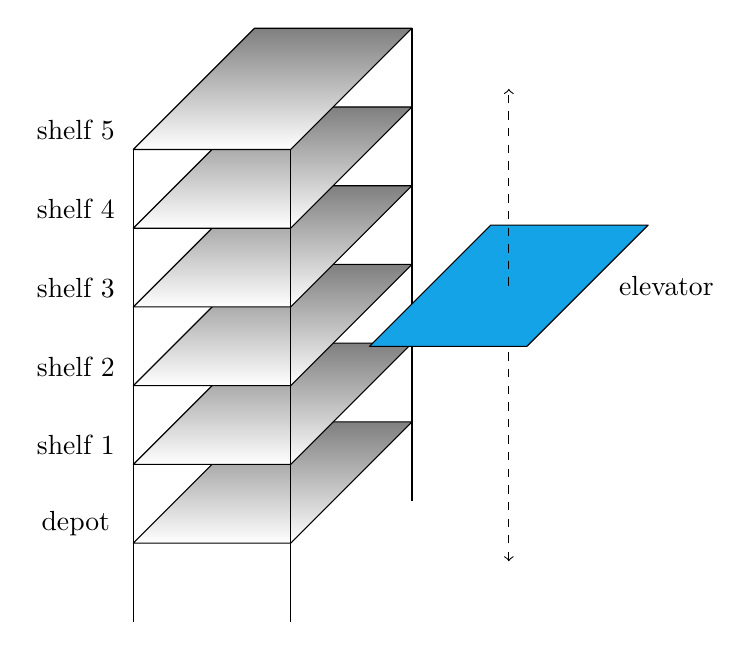
\begin{tikzpicture}
    \tikzset{shelf/.style={fill=lightgray,draw=black,line join=round}}
    \tikzset{elevator/.style={fill=Cerulean,draw=black,line join=round}}
    \begin{scope}[canvas is xz plane at y=0]
        \path[shelf,shade] (0,0) rectangle (2,4);
    \end{scope}
    \begin{scope}[canvas is xz plane at y=1]
        \path[shelf,shade] (0,0) rectangle (2,4);
    \end{scope}
    \begin{scope}[canvas is xz plane at y=2]
        \path[shelf,shade] (0,0) rectangle (2,4);
    \end{scope}
    \begin{scope}[canvas is xz plane at y=3]
        \path[shelf,shade] (0,0) rectangle (2,4);
    \end{scope}
    \begin{scope}[canvas is xz plane at y=4]
        \path[shelf,shade] (0,0) rectangle (2,4);
    \end{scope}
    \begin{scope}[canvas is xz plane at y=5]
        \path[shelf,shade] (0,0) rectangle (2,4);
    \end{scope}
    \begin{scope}[canvas is xy plane at z=0]
        \draw (2,-1) -- (2,5);
    \end{scope}
    \begin{scope}[canvas is xy plane at z=4]
        \draw (2,-1) -- (2,5);
    \end{scope}
    \begin{scope}[canvas is xy plane at z=4]
        \draw (0,-1) -- (0,5);
    \end{scope}
    \node[yshift=-15] at (-1.5,0,2) {depot};
    \node[yshift=-15] at (-1.5,1,2) {shelf 1};
    \node[yshift=-15] at (-1.5,2,2) {shelf 2};
    \node[yshift=-15] at (-1.5,3,2) {shelf 3};
    \node[yshift=-15] at (-1.5,4,2) {shelf 4};
    \node[yshift=-15] at (-1.5,5,2) {shelf 5};

    \begin{scope}[canvas is xy plane at z=2]
        \draw[<-,dashed] (4,-1) -- (4,2.5);
    \end{scope}
    \begin{scope}[canvas is xz plane at y=2.5]
        \draw[elevator] (3,0) rectangle (5,4);
    \end{scope}
    \begin{scope}[canvas is xy plane at z=2]
        \draw[->,dashed] (4,2.5) -- (4,5);
    \end{scope}
    \node at (6,2.5,2) {elevator};
\end{tikzpicture}
        \caption{Schematic representation of a shelf tower with five shelves plus the depot, serviced by an elevator.}\label{fig:shelf-stack}
    \end{figure}

    A VF tower is composed of stacked shelves in which a planner places trays containing crops.
    Each tray will spend some time in this system, until the crops it contains are ready to be harvested.
    Each shelf can host one tray at a time and, after a tray leaves a shelf, another one can take its place.
    Trays become available from a ``depot'' at the bottom, spend the required amount of time in a shelf and, at the end of the crop's growth period, return to the depot.
    In an automatic vertical farm, an elevator moves the trays between the depot and the shelves.
    \Cref{fig:shelf-stack} gives a schematic representation of a stack with five shelves (plus the depot) serviced by an elevator.
    A human operator brings a seeded tray to the depot, so that the elevator can place it into a shelf.
    At the end of the growth cycle of the crop, the elevator brings the tray down and the operator picks it up from the depot and moves it into an area where the crop will be harvested.
    
    The elevator also services the trays performing activities such as watering and monitoring.
    For example, it can take pictures that a computer vision algorithm processes to ensure crops are growing well and aren't affected by pests.
    Each tray has an associated list of tasks, and each task requires that the elevator travels to the corresponding shelf and spends some time there.
    
    Each tray has a start time window during which it must be picked up at the depot, to be placed on its assigned shelf.
    We define the time at which the elevator picks up the tray to bring it to its shelf as the tray's {\em start time}.
    There are also time windows related to each task and to the final pick up of the tray, but these are relative to the tray's start time.
    For example, if a tray has a start time window of one day (from hour 0 to 24), it can be brought to its shelf at hour 12.
    Then, if it must be watered after 6--8 hours from growth start, this would translate into a task time window spanning from hour 18 to hour 20.
    
    A computer system is in charge of sequencing the tasks and correspondingly move the elevator.
    The objective of the system is to minimise the energy consumption of the elevator, making sure that all tasks are performed within their time windows.
    The elevator uses energy to travel between shelves.
    Therefore, the energy minimisation objective translates into the minimisation of the distance travelled by the elevator.
    
    In the problem considered in this paper, another subsystem in the control software of the tower has already taken care of assigning each tray to the shelf it will occupy (see \Cref{sec:conclusion} for possible extensions).
    The elevator must then transport each tray to and from its assigned shelf, and visit the trays to perform the given list of tasks.
    The elevator can carry out tasks associated with different trays in any order, as long as the time windows are respected.
    On the other hand, tasks associated with the same tray must be carried out in the given order.
    
    The objective of the problem is to determine a sequence of operations which minimises the travel distance of the elevator.
    Because the travel time of the elevator (a few seconds) is negligible compared to the time it must spend at the shelves to perform the tasks (several minutes), we can disregard it when timing the operations.
    
    \section{Literature review}\label{sec:literature_review}
    
    There is a limited but growing amount of literature on the topic of the optimisation of VF.
    Two of the earliest works, by \textcite{yang2012vf} and \textcite{potts2017vf}, respectively, are only available as short abstracts in conference proceedings.
    
    \textcite{yang2012vf} study the problem of selecting and scheduling a mix of crops to grow in a VF system, at a tactical level.
    The objective is to maximise profits, keeping into account that the price of each crop fluctuates during the year.
    The fluctuation is due to the possibility of growing some of the crops using open-air agriculture, which is highly seasonal.
    Therefore, it is more profitable to harvest a crop in the VF system during the period of the year when it is not available using open-air agriculture.
    The author propose a small case study with a 2-year time horizon and 13 possible crops, which is solved using a MIP.
    
    The problem of meeting as much demand as possible using crops grown in a VF cabinet was studied by~\textcite{potts2017vf}.
    The authors consider a stack of shelves similar to the one presented in \Cref{fig:shelf-stack}, although smaller in scale: their proposed use-case is a cabinet placed directly at consumer site (e.g., at a restaurant or a supermarket).
    In their settings, the capacity of each shelf and the growth speed of each crop are determined by a set of growth conditions, which the operator can change.
    For example, each crop can grow on a different growth medium, receive more or less light, water, etc.
    Using these factors to influence the length of the growth cycles, \citeauthor{potts2017vf} minimise the amount of unmet demand, weighted by crop prices.
    The authors propose a heuristic rolling-horizon algorithm.
    
    \textcite{yang2019} expand on \parencite{yang2012vf}, considering again the problem of selecting and scheduling crop growth in a VF system.
    The authors consider a setting in which crops receive sunlight (as opposed to artificial light) and the amount of light depends on the shelf's position and on whether the system operator installs rooftop solar panels, which obstruct the glass ceiling.
    Similar to \parencite{yang2012vf}, the author aim at maximising the profit considering the seasonal variability of crop prices.
    Additionally, they introduce crop adjacency considerations, which make it more desirable for crops of the same family to grow on adjacent shelves.
    The MIP formulation proposed by the authors is not able to scale to realistic-size instances and, therefore, they implement a greedy heuristic which provides solutions for time horizons of up to 50 months.
    
    Recently, \textcite{santini2021vf} considered the problem of planning the production of crops on VF cabinets.
    The authors consider a system in which crops grow under controlled conditions (soil, water, light, CO\textsubscript{2} levels, etc.) which can change day-by-day and on a shelf-by-shelf level.
    They propose four objective functions which a planner might want to minimise: the amount of unmet demand (if it's not possible to satisfy the entire demand with the available infrastructure), the number of tray movements (trays are allowed to move from a shelf to another one during their growth), the number of shelf reconfigurations (i.e., the number of time the operator changes growth conditions for a shelf), and the number of shelves used.
    They prove that the problem is \(\mathcal{NP}\)-complete and provide MIP models for the four versions.
    The models are tested on instances with up to 6 crops, 12 shelves, and a time horizon of 100 days.
    Their results show that the choice of the objective function heavily influences both the computational performance of the model and the characteristics of the solution, hinting that a multi-objective approach could be useful to build a real-world decision support system.
    
    In another recent paper, \textcite{cetegen2021vf} present a robust optimisation model to design a VF system and schedule crop growth.
    The authors aim at building a portfolio of crops to grow, to minimise the risk of economic losses under worst-case market scenarios.
    Because controlled-environment agricultural techniques such as VF virtually eliminate risks on the grower's side (bad weather, pests, etc.) the author consider risks coming from the market's side, i.e., demand and price variability.
    Using a cutting-plane method to solve a semi-infinite programme with semi-infinite constraints, the authors apply their algorithm to two case studies, validating the economic viability of using VF to grow crops such as lettuce, spinach, tomatoes, strawberries and mushrooms.
    
    We also highlight a recent Master's thesis \parencite{vfms2021}, which deals with task scheduling in a semi-automatic VF plant factory.
    The objective considered is the minimisation of the makespan of tasks to be performed by sensors and actuators on the crop trays growing in the VF system.
    Such objective allows the authors to model the problem as a Flexible Job-Shop Scheduling Problem and use a variant of the Genetic Algorithm by \textcite{fjsp2008} for its solution.
    
    Finally, we remark that our problem has a superficial similarity with the Travelling Salesman Problem with Time Windows (TSPTW): if the task time windows were absolute rather than relative to the planting time, our problem could be seen as an extension of a 1-dimensional TSPTW.
    The current literature, however, does not present any work neither on routing problems in which the time window of a customer is relative to the visit time of another customer, nor on 1-dimensional special cases of routing problems with time windows.
    
    \section{Problem formalisation}\label{sec:formalisation}
    
    Consider a tower with \(n\) shelves, making up set \(S = \{1, \ldots, n\}\).
    We denote the bottom depot as \(0\) and the set of all shelves plus the depot as \(S' = \{0\} \cup S\).
    During the planning horizon, \(m\) trays will be placed on the shelves; we denote them as \(T = \{1, \ldots, m\}\).
    The time horizon itself is discretised in time intervals and denoted as \(\Omega = \{1, \ldots, \omega\}\).
    
    Each tray \(t \in T\) has a start time window \(\big[ \ubar{w}^0_t, \bar{w}^0_t \big]\) (with \(\ubar{w}^0_t, \bar{w}^0_t \in \Omega\) and \(\ubar{w}^0_t \leq \bar{w}^0_t\)) during which it must be picked up at the depot.
    The elevator must stay at the depot for \(d^0_t \geq 1\) further time units when picking up the tray, to allow loading operations.
    Furthermore, there is a list of \(l_t\) tasks which the elevator must perform on tray \(t\); the set of these tasks is denoted as \(J_t = \{ 1, \ldots, l_t \}\).
    Each task \(j \in J_t\) has an associated (relative) time window \(\big[ \ubar{w}^j_t, \bar{w}^j_t \big]\) during which the elevator must start the task, and a duration \(d^j_t \geq 1\) during which the elevator cannot move away from the shelf containing \(t\).
    Finally, we denote with \(\big[ \ubar{w}^{l_t+1}_t, \bar{w}^{l_t+1}_t \big]\) the (relative) time window during which the elevator must pick up tray \(t\) and bring it back to the depot, and with \(d^{l_1+1}_t \geq 1\) the further time the elevator must spend at the depot after bringing the tray, to allow unloading operations.
    Time windows for tasks \(> 0\) are relative to the time in which the elevator reached the depot to pick up the tray when performing task \(0\).
    We define the set of extended tasks as \(J_t' = \{0\} \cup J_t \cup \{l_t + 1\}\).
    
    We allow time windows to overlap for a given tray, i.e., it could happen that \(\bar{w}^j_t + d^j_t \geq \ubar{w}^{j+1}_t,\; \forall j \in \{ 1, \ldots, l_t \}\).
    However, to ensure the proper growth of the crops, we require tasks to be executed in their given order, i.e., for a given tray, a task \(j+1\) cannot be performed before task \(j\).
    
    It is also possible that the allowed ``shelf life'' of a tray (i.e., the moments in which it is allowed to be present on its assigned shelf) can overlap with that of another tray assigned to the same shelf.
    In other words, given two trays \(t_1, t_2\) such that both are assigned to the same shelf, it can happen that
    \begin{equation}
        \bar{w}^0_{t_1} + \bar{w}^{l_{t_1}+1}_{t_1} \geq \ubar{w}^0_{t_2}\textrm{.}\label{eq:overlap}
    \end{equation}
    However, the two intervals \([\bar{w}^0_{t_1}, \ubar{w}^0_{t_1} + \ubar{w}^{l_{t_1}+1}_{t_1}]\) and \([\bar{w}^0_{t_2}, \ubar{w}^0_{t_2} + \ubar{w}^{l_{t_2}+1}_{t_2}]\) (if non-empty) cannot overlap, as they represent the time instants in which the trays are required to be on the shelf and two trays cannot occupy the same shelf at the same time.
    
    Because all shelves are equally spaced in the silo, the distance travelled by the elevator when moving from a shelf \(s_1 \in S'\) to another shelf \(s_2 \in S'\) can be easily expressed as \(c_{s_1,s_2} = c_{s_2,s_1} = |s_1 - s_2|\).
    We also denote the shelf assigned to a tray \(t \in T\) as \(s(t) \in S\).
    
    We define the Vertical Farming Elevator Energy Minimisation Problem (VFEEMP) as the problem of deciding in which order to perform the tasks, to minimise the distance travelled by the elevator.
    The VFEEMP superficially resembles a 1-dimensional Travelling Salesman Problem with Time Windows.
    However, in our problem and differently from any other problem we are aware of, most time windows are {\em relative} and depend on other decisions taken by the planner, namely the start time of the planting task.
    As such, the VFEEMP does not seem to be neither a special case nor a generalisation of other known optimisation problems and, thus, a first interesting question regards its computational complexity.
    \Cref{thm:np-complete} answer this question, proving that the decision version of the VFEEMP is \(\mathcal{NP}\)-complete.
    
    \begin{theorem}\label{thm:np-complete}
        Let {\sc VFEEMP-Decision} be the decision problem which asks whether there is a solution to the VFEEMP of cost at most \(x\), for a given \(x \in \mathbb{R}^+_0\).
        Then {\sc VFEEMP-Decision} is \(\mathcal{NP}\)-complete.
    \end{theorem} 
    \begin{proof}
        We prove the thesis by proving a stronger statement: that determining whether VFEEMP is feasible is itself \(\mathcal{NP}\)-complete.
        This clearly implies that {\sc VFEEMP-Decision} is \(\mathcal{NP}\)-complete.
    
        Consider an instance of the \(\mathcal{NP}\)-complete {\sc SubsetSum} problem: given a set of \(n\) positive integers \(\mathcal{B} = \{b_1, \dots, b_{n}\}\) and a positive integer \(c\), the problem asks to determine whether there is a subset \(\mathcal{S} \subseteq \mathcal{B}\) such that \(\sum_{b \in \mathcal{S}} b = c\).
        We show how to create an instance of the VFEEMP such that, if the instance is feasible then {\sc SubsetSum} has answer {\sc Yes} and, otherwise, it has answer {\sc No}.
        
        The main idea is to first transform the {\sc SubsetSum} instance by multiplying each \(b_i\) and \(c\) by 2, to only deal with even numbers.
        Next, we build an instance in which each tray uses \(2 b_i\) units of elevator time, in which the elevator can never be idle, and in which there is a special tray which must be picked up at time \(2c+1\).
        In this way, being able to service a subset of trays before time \(2c+1\) corresponds to finding a subset of the (doubled) integers summing up to \(2c\), i.e., a set of the original integers which sums to \(c\).
        
        Formally, we create the VFEEMP instance as follows: let \(B = 2 \sum_{i=1}^n b_i\), set the number of shelves to 1, the number of trays to \(n+1\) and the time horizon to \(\Omega = \{1,\ldots, B+4\}\).
        Each of the first \(i = 1,\dots,n\) trays has:
        \begin{itemize}[nosep]
            \item Start time window \(\big[1,  B - 2b_i \big]\) and \(d^0_i = b_i\).
            \item No intermediate tasks.
            \item End time window \(\big[b_i, b_i\big]\) and \(d^1_i = b_i\).
        \end{itemize}
        Tray \(n+1\) has:
        \begin{itemize}[nosep]
            \item Start time window \(\big[2c+1, 2c+1\big]\) and \(d^0_{n+1} = 1\).
            \item A unique task of duration \(d^1_{n+1} = 1\) with relative time window \(\big[1,1\big]\).
            \item End time window \(\big[1,1\big]\) and \(d^2_{n+1} = 1\). 
        \end{itemize}
        Because of the characteristics of the instance, finding a solution amounts to determining a permutation of the indices \(\{1,\ldots,n+1\}\) indicating in which order the trays occupy the only shelf.
        The upper bounds on the start time windows of the shelves imply that the elevator cannot be idle at any time in a feasible solution, or there would be no time to service all trays: each tray \(i \neq n+1\) requires \(2 b_i\) units of time and tray \(n+1\) requires 3 time intervals, so that the elevator must be busy up to the last time interval \(B+4\).
        
        If VFEEMP is feasible, let \((\pi_1, \ldots, \pi_{n+1})\) be the permutation corresponding to a solution and let \(j\) be the index such that \(\pi_j = n+1\).
        Then, because each tray \(i\) consumes exactly \(2b_i\) units of elevator time and because tray \(n+1\) must be picked up exactly at time \(2c+1\), then we must have that \(\sum_{i=1}^{j-1} 2b_i = 2c\).
        This implies \(\sum_{i=1}^{j-1} b_i = c\) and, therefore, {\sc SubsetSum} has answer {\sc Yes}.
        \Cref{fig:subsetsum} depicts such a situation.
        
        Noting that the above VFEEMP instance can be built in linear time in the size \(n\) of the {\sc SubsetSum} instance concludes the proof.
    \end{proof}
    
    \begin{figure}\centering
        \resizebox{\textwidth}{!}{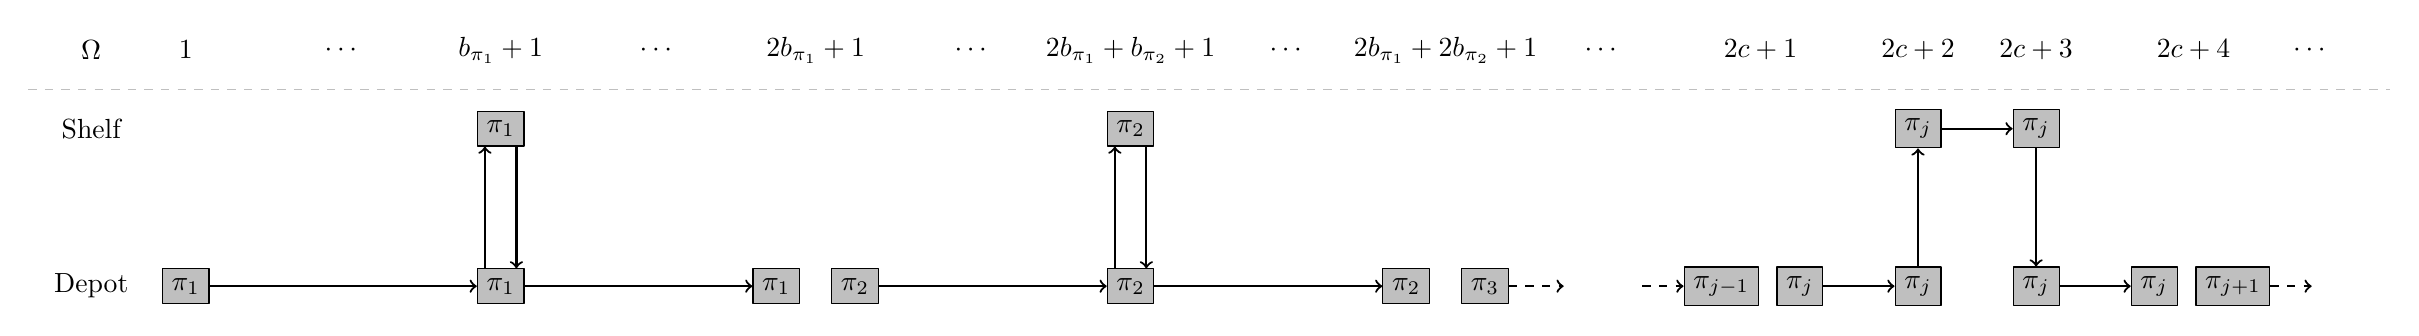
\begin{tikzpicture}
    \node[align=right] at (-.2,-1) {Depot};
    \node[align=right] at (-.2,1) {Shelf};
    \node[align=right] at (-.2,2) {$\Omega$};
    
    \draw[dashed,lightgray] (-1,1.5) -- (29,1.5);
    
    \node at (1,2) {1};
    \node at (3,2) {$\cdots$};
    \node at (5,2) {$b_{\pi_1} + 1$};
    \node at (7,2) {$\cdots$};
    \node at (9,2) {$2 b_{\pi_1} + 1$};
    \node at (11,2) {$\cdots$};
    \node at (13,2) {$2 b_{\pi_1} + b_{\pi_2} + 1$};
    \node at (15,2) {$\cdots$};
    \node at (17,2) {$2 b_{\pi_1} + 2 b_{\pi_2} + 1$};
    \node at (19,2) {$\cdots$};
    \node at (21,2) {$2c + 1$};
    \node at (23,2) {$2c + 2$};
    \node at (24.5,2) {$2c + 3$};
    \node at (26.5,2) {$2c + 4$};
    \node at (28,2) {$\cdots$};
    
    \tikzset{albrect/.style={fill=lightgray,draw=black,line join=round}}
    
    \node[albrect] (p1d) at (1,-1) {$\pi_1$};
    \node[albrect] (p5d) at (5,-1) {$\pi_1$};
    \node[albrect] (p5s) at (5,1) {$\pi_1$};
    \node[albrect] (p9d) at (8.5,-1) {$\pi_1$};
    
    \node[albrect] (p9d2) at (9.5,-1) {$\pi_2$};
    \node[albrect] (p13d) at (13,-1) {$\pi_2$};
    \node[albrect] (p13s) at (13,1) {$\pi_2$};
    \node[albrect] (p17d) at (16.5,-1) {$\pi_2$};
    
    \node[albrect] (p17d2) at (17.5,-1) {$\pi_3$};
    
    \node[albrect] (p21d) at (20.5,-1) {$\pi_{j-1}$};
    
    \node[albrect] (p21d2) at (21.5,-1) {$\pi_j$};
    \node[albrect] (p22d) at (23,-1) {$\pi_j$};
    \node[albrect] (p22s) at (23,1) {$\pi_j$};
    \node[albrect] (p24s) at (24.5,1) {$\pi_j$};
    \node[albrect] (p24d) at (24.5,-1) {$\pi_j$};
    \node[albrect] (p25d) at (26,-1) {$\pi_j$};
    
    \node[albrect] (p25d2) at (27,-1) {$\pi_{j+1}$};
    
    \draw[->,thick] (p1d.east) -- (p5d.west);
    \draw[->,thick] ($(p5d.north) - (.2,0)$) -- ($(p5s.south) - (.2,0)$);
    \draw[->,thick] ($(p5s.south) + (.2,0)$) -- ($(p5d.north) + (.2,0)$);
    \draw[->,thick] (p5d.east) -- (p9d.west);
    
    \draw[->,thick] (p9d2.east) -- (p13d.west);
    \draw[->,thick] ($(p13d.north) - (.2,0)$) -- ($(p13s.south) - (.2,0)$);
    \draw[->,thick] ($(p13s.south) + (.2,0)$) -- ($(p13d.north) + (.2,0)$);
    \draw[->,thick] (p13d.east) -- (p17d.west);
    
    \draw[->,thick,dashed] (p17d2.east) -- (18.5,-1);
    
    \draw[->,thick,dashed] (19.5,-1) -- (p21d.west);
    
    \draw[->,thick] (p21d2.east) -- (p22d.west);
    \draw[->,thick] (p22d.north) -- (p22s.south);
    \draw[->,thick] (p22s.east) -- (p24s.west);
    \draw[->,thick] (p24s.south) -- (p24d.north);
    \draw[->,thick] (p24d.east) -- (p25d.west);
    
    \draw[->,thick,dashed] (p25d2) -- (28,-1);
\end{tikzpicture}}
        \caption{Visualisation of a feasible VFEEMP transformed from {\sc SubsetSum}.}\label{fig:subsetsum}
    \end{figure}
    
    \section{Model formulation}\label{sec:formulations}
    
    In this section, we propose four formulations for the VFEEMP.
    The first three are based on MIP: the first uses a polynomial number of variables and disjunctive constraints; the second one uses a pseudo-polynomial number of variables; the third one is a hybrid  which only uses binary variables from the first and the second formulation.
    Finally, the fourth formulation is based on CP.

    \subsection{A model with disjunctive constraints}\label{ssec:formulation-M1}
    
    Before presenting this model, we add to \(\Omega\) a dummy time interval \(0\), and to \(T\) a dummy tray with index \(0\), assigned to the depot with start time window \(\big[0, 0\big]\) and \(d^0_0 = 1\), no intermediary tasks, and end time window \(\big[\omega,\omega\big]\) and \(d^1_0 = 1\).
    The dummy tray models the fact that the elevator starts and must return to the depot.
    
    We introduce variables \(y_{t_1,j_1,t_2,j_2} \in \{0,1\}\), for \(t_1, t_2 \in T\), \(j_1 \in J_{t_1}'\) and \(j_2 \in J_{t_2}'\) (with \(j_1 \neq j_2\) when \(t_1 = t_2\)).
    Variable \(y_{t_1,j_1,t_2,j_2}\) takes value 1 iff the elevator performs task \(j_1\) on tray \(t_1\) and, immediately afterwards, it performs task \(j_2\) on tray \(t_2\).
    Recall that the assignment of trays to shelves is given, and that we denote with \(s(t) \in S\) the shelf assigned to tray \(t \in T\).
    We denote with \(c(y_{t_1,j_1,t_2,j_2}) \in \mathbb{N}\) the travel cost associated to variable \(y_{t_1,j_1,t_2,j_2}\).
    To assign a value to \(c(\cdot)\), we consider the following cases (see \Cref{fig:y-cases}):
    \begin{alignat}{3}
    & j_1 = 0           && j_2 = 0           && c(y_{t_1,0,t_2,0}) = s(t_1) + s(t_2)                           \label{eq:c_case1}\\
    & j_1 = 0           && j_2 \in J_{t_2}   && c(y_{t_1,0,t_2,j_2}) = |s(t_1) - s(t_2)|                \label{eq:c_case2}\\
    & j_1 = 0           && j_2 = l_{t_2} + 1 && c(y_{t_1,0,t_2,l_{t_2}+1}) = |s(t_1) - s(t_2)| + s(t_2) \label{eq:c_case3}\\
    & j_1 \in J_{t_1}   && j_2 = 0           && c(y_{t_1,j_1,t_2,0}) = s(t_1) + s(t_2)                           \label{eq:c_case4}\\
    & j_1 \in J_{t_1}   && j_2 \in J_{t_2}   && c(y_{t_1,j_1,t_2,j_2}) = |s(t_1) - s(t_2)|                       \label{eq:c_case5}\\
    & j_1 \in J_{t_1}   && j_2 = l_{t_1} + 1 && c(y_{t_1,y_1,t_1,l_{t_2}+1}) = |s(t_1) - s(t_2)| + s(t_2)        \label{eq:c_case6}\\
    & j_1 = l_{t_1} + 1 && j_2 = 0           && c(y_{t_1,l_{t_1}+1,t_2,0}) = s(t_2)                     \label{eq:c_case7}\\
    & j_1 = l_{t_1} + 1 && j_2 \in J_2       && c(y_{t_1,l_{t_1}+1,t_2,j_2}) = s(t_2)                   \label{eq:c_case8}\\
    & j_1 = l_{t_1} + 1\quad && j_2 = l_{t_2} + 1\quad && c(y_{t_1,l_{t_1}+1,t_2,l_{t_2}+1}) = 2 s(t_2)\mathrm{.} \label{eq:c_case9}
    \end{alignat}
    
    Let us also introduce the following notation:
    \begin{align}
        \alpha_{tj} &= \begin{cases}
            \ubar{w}^0_t & \text{ if } j = 0 \\
            \ubar{w}^0_t + \ubar{w}^j_t & \text{ otherwise,}
        \end{cases} \\
        \beta_{tj} &= \begin{cases}
            \bar{w}^0_t & \text{ if } j = 0 \\
            \bar{w}^j_t + \bar{w}^0_t & \text{ otherwise.}
        \end{cases}
    \end{align}
    In other words, \(\alpha_{tj}\) and \(\beta_{tj}\) are the earliest and latest time intervals at which task \(j \in J'_t\) can start.
    We now notice that not all possible quadruples \((t_1, j_1, t_2, j_2)\) are valid indices for variables \(y\):
    \begin{itemize}
        \item If \(t_2 = 0\) and \(j_2 = 0\), then no indices \(t_1, j_1, t_2, j_2\) can be valid, as the start task of the dummy tray cannot have any predecessor.
        \item Analogously, if \(t_1 = 0\) and \(j_1 = 1\), then no indices \(t_1, j_1, t_2, j_2\) can be valid, because the end task of the dummy tray cannot have any successor. 
        \item We can also omit indices which would result in time window violations.
        Specifically, if \(\beta_{t_2 j_2} < \alpha_{t_1 j_1} + d_{t_1}^{j_1}\) then task \(j_2\) must be performed before task \(j_1\) and cannot be its successor.
        Therefore, we need not consider indices \(t_1, j_1, t_2, j_2\) satisfying the above condition.
        \item If \(t_1 = t_2\), then only indices for which \(j_2 = j_1 + 1\) are valid; otherwise, tasks would be performed out-of-order for that tray.
        \item If there is another task \(j_3 \in J'_{t_3}\) (for some tray \(t_3 \in T\)) which must take place between \(j_1\) and \(j_2\), then these two tasks cannot happen in succession.
        More precisely, indices \(t_1,j_1,t_2,j_2\) are not valid if
        \begin{equation*}
            \exists t_3 \in T, \; j_3 \in J'_{t_3} \ : \ \alpha_{t_3 j_3} + d_{t_3}^{j_3} > \beta_{t_1 j_1} \text{ and } \beta_{t_3 j_3} < \alpha_{t_2 j_2} + d_{t_2}^{j_2}\textrm{.}
        \end{equation*}
    \end{itemize}
    Let us denote with \(V\) the set of valid indices for variables \(y\), i.e., the set of all quadruples \((t_1, j_1, t_2, j_2)\) which are not excluded by one of the above conditions.
    
    \begin{figure}[tbp]\centering
        \captionsetup[subfigure]{labelformat=empty,aboveskip=-.5em}
\begin{subfigure}[b]{0.3\textwidth}\centering
    \begin{equation*}
        \to 0 \to s(t_1) \to 0 \to s(t_2) \to
    \end{equation*}
    \caption{Case \eqref{eq:c_case1}}
\end{subfigure}%
\hfill
\begin{subfigure}[b]{0.3\textwidth}\centering
    \begin{equation*}
        \to 0 \to s(t_1) \to s(t_2) \to
    \end{equation*}
    \caption{Case \eqref{eq:c_case2}}
\end{subfigure}%
\hfill
\begin{subfigure}[b]{0.3\textwidth}\centering
    \begin{equation*}
        \to 0 \to s(t_1) \to s(t_2) \to 0 \to
    \end{equation*}
    \caption{Case \eqref{eq:c_case3}}
\end{subfigure}

\begin{subfigure}[b]{0.3\textwidth}\centering
    \begin{equation*}
        \to s(t_1) \to 0 \to s(t_2) \to
    \end{equation*}
    \caption{Case \eqref{eq:c_case4}}
\end{subfigure}%
\hfill
\begin{subfigure}[b]{0.3\textwidth}\centering
    \begin{equation*}
        \to s(t_1) \to s(t_2) \to
    \end{equation*}
    \caption{Case \eqref{eq:c_case5}}
\end{subfigure}%
\hfill
\begin{subfigure}[b]{0.3\textwidth}\centering
    \begin{equation*}
        \to s(t_1) \to s(t_2) \to 0 \to
    \end{equation*}
    \caption{Case \eqref{eq:c_case6}}
\end{subfigure}

\begin{subfigure}[b]{0.3\textwidth}\centering
    \begin{equation*}
        \to s(t_1) \to 0 \to s(t_2) \to
    \end{equation*}
    \caption{Case \eqref{eq:c_case7}}
\end{subfigure}%
\hfill
\begin{subfigure}[b]{0.3\textwidth}\centering
    \begin{equation*}
        \to s(t_1) \to 0 \to s(t_2) \to
    \end{equation*}
    \caption{Case \eqref{eq:c_case8}}
\end{subfigure}%
\hfill
\begin{subfigure}[b]{0.3\textwidth}\centering
    \begin{equation*}
        \to s(t_1) \to 0 \to s(t_2) \to 0 \to
    \end{equation*}
    \caption{Case \eqref{eq:c_case9}}
\end{subfigure}
        \caption{Possible cases for the costs associated with variables \(y_{t_1,j_1,t_2,j_2}\). Each case depicts more movements than those considered in the corresponding cost; this is because doing otherwise would lead to count some movement costs twice.}\label{fig:y-cases}
    \end{figure}

    We also consider continuous variables \(s_{tj}\) indicating the starting time of task \(j\) on tray \(t\) (\(t \in T, j \in J'_{t}\)).
    Finally, let \(\Delta_{t_1 t_2} \in \{0,1\}\) be a binary variable defined for each pair of trays \(t_1, t_2 \in T\) such that \(s(t_1) = s(t_2)\).
    It will take value 1 iff tray \(t_1\) is placed on the shelf before tray \(t_2\).
    The VFEEMP can then be modelled with the following MIP, which we denote {\bf M1}:
    \begin{alignat}{3}
    & \min\quad  && \sum_{(t_1, j_1, t_2, j_2) \in V} c(y_{t_1,j_1,t_2,j_2}) \cdot y_{t_1,j_1,t_2,j_2} \label{M1:obj}\\
    & \text{s.t.} \quad && \sum_{(t_1, j_1, t, j) \in V} y_{t_1,j_1,t,j} = 1 && \forall t \in T, \; \forall j \in J'_t, (t, j) \neq (0, 0) \label{M1:dotask} \\
    & \quad && \sum_{(0, 0, t, j) \in V} y_{0,0,t,j} = 1 \label{M1:dummy1}  \\
    & \quad && \sum_{(t_1, j_1, t, j) \in V} y_{t_1,j_1,t,j} = \sum_{(t, j, t_2, j_2) \in V} y_{t,j,t_2,j_2} && \forall t \in T \setminus{\{0\}}, \; \forall j \in J'_{t} \label{M1:predsucc} \\
    & \quad && s_{t0} \geq \ubar{w}^0_t && \forall t \in T \label{M1:pickup_lb}\\
    & \quad && s_{t0} \leq \bar{w}^j_0 && \forall t \in T \label{M1:pickup_ub}\\
    & \quad && s_{tj} \geq s_{t0} + \ubar{w}^j_t && \forall t \in T, \; \forall j \in J'_{t} \setminus\{0\} \label{M1:task_lb}\\
    & \quad && s_{tj} \leq s_{t0} + \bar{w}^j_t && \forall t \in T, \; \forall j \in J'_{t} \setminus\{0\} \label{M1:task_ub}\\
    & \quad && s_{tj} \geq s_{t,j-1} + d^{j-1}_{t} && \forall t \in T, \; \forall j \in J'_{t} \setminus\{0\} \label{M1:task_lb2}\\
    & \quad && s_{t_2 j_2} \geq s_{t_1 j_1} + d^{j_1}_{t_1} - M (1 - y_{t_1,j_1,t_2,j_2})  \label{M1:duration} && \forall (t_1, j_1, t_2, j_2) \in V \\
    & \quad && s_{t_1 0} \geq s_{t_2, l_{t_2} + 1} + d_{t_2}^{l_{t_2}+1} - M \cdot \Delta_{t_1 t_2} && \forall t_1, t_2 \in T, \; s(t_1) = s(t_2), \; t_1 \neq t_2 \label{M1:set_Delta} \\
    & \quad && \Delta_{t_1 t_2} + \Delta_{t_2 t_1} \leq 1 && \forall t_1, t_2 \in T, \; s(t_1) = s(t_2), \; t_1 < t_2 \label{M1:sequence} \\ 
    & \quad && y_{t_1,j_1,t_2,j_2} \in \{0,1\} && \forall (t_1, j_1, t_2, j_2) \in V \label{M1:def_y} \\
    & \quad && s_{tj} \geq 0  && \forall t \in T, \; \forall j \in J'_{t} \label{M1:def_s} \\
    & \quad && \Delta_{t_1 t_2} \in \{0, 1\} && \forall t_1, t_2 \in T \; : \; s(t_1) = s(t_2), \; t_1 \neq t_2 \label{M1:def_Delta}
    \end{alignat}
    Objective function \eqref{M1:obj} minimises the travel cost of the elevator.
    Constraints \eqref{M1:dotask} ensure that every task of every tray (excluding the start task of the dummy tray) has a predecessor and, therefore, is processed.
    Constraints \eqref{M1:dummy1} force the elevator to process the start task of the dummy tray, while constraints \eqref{M1:predsucc} make sure that every task (excepted those associated with the dummy tray) has a direct predecessor and a direct successor.
    Constraints \eqref{M1:pickup_lb} and \eqref{M1:pickup_ub} make sure that each tray is picked up during its associated (absolute) start time window, while constraints \eqref{M1:task_lb} and \eqref{M1:task_ub} ensure that every task other than the start task takes place during its associated (relative) time window.
    Constraints \eqref{M1:task_lb2} force tasks associated to the same tray to be scheduled in the given order and are necessary because task time windows can overlap.
    Constraints \eqref{M1:duration}, in which \(M\) is a sufficiently large number, force the starting time of any task to be not earlier than the starting time plus the duration of its predecessor.
    The tightest value for \(M\) is \(\beta_{t1 j1} + d_{t_1}^{j_1} - \alpha_{t_2 j_2}\).
    Constraints similar to \eqref{M1:duration} are also used in the literature on routing problems with time windows to sequence customer visits \parencite[see, e.g., constraint (14) of][]{KARA20151026} and in scheduling to sequence tasks \parencite[see, e.g., constraint (5) of][]{santini2015note}.
    Constraints \eqref{M1:set_Delta} link variables \(s\) and \(\Delta\) (again, using a sufficiently large number \(M\)), while constraints \eqref{M1:sequence} ensure that no two trays occupy the same shelf at the same time.
    The tightest value for \(M\) in \eqref{M1:set_Delta} is \(\beta_{t_2, l_{t_2} + 1} + d_{t_2}^{l_{t_2} + 1} - \alpha_{t_1 0}\).
    Variables \(\Delta\) and constraints \eqref{M1:set_Delta}--\eqref{M1:sequence} are required because tray shelf lives can overlap and, therefore, the model must determine a processing order for trays on the same shelf.
    Finally, \eqref{M1:def_y}, \eqref{M1:def_s}, and \eqref{M1:def_Delta} are variable domain definitions.
    
    \subsubsection{Valid inequalities}\label{sssec:M1-valid}
    
    We introduce in the following sets of valid inequalities for model \textbf{M1}.
    Their impact is tested by means of computational experiments presented in \Cref{ssec:comp-res-syn}.
    
    \paragraph{Task incompatibility (\textsc{TaskInc}).}
    The task incompatibility considerations we use to reduce the set of feasible indices for variables \(y\) can be extended to more than two tasks at a time.
    For example, the following inequality is valid for model \textbf{M1}:
    \begin{equation}
        y_{t_1,j_1,t_2,j_2} + y_{t_2,j_2,t_3,j_3} \leq 1 \quad \forall (t_1, j_1, t_2, j_2), (t_2, j_2, t_3, j_3) \in V \; : \; \beta_{t_3 j_3} < \alpha_{t_1 j_1} + d_{t_1}^{j_1} + d_{t_2}^{j_2}\mathrm{.}\label{M1:valid-ineq1}
    \end{equation}
    In this case, \eqref{M1:valid-ineq1} states that tasks \(j_1\), \(j_2\) and \(j_3\) cannot be performed in the given order, due to their time windows and durations.
    Although one could consider similar clique inequalities for larger sets of mutually incompatible tasks, detecting such sets becomes harder while the constraints would be less likely to be active.
    For this reason, we only add inequalities of type \eqref{M1:valid-ineq1} to model \textbf{M1}.
    
    \paragraph{Force task sequence (\textsc{TaskSeq}).}
    While constraint \eqref{M1:valid-ineq1} {\em excludes} incompatible tasks, we next present a constraint aimed at {\em forcing} tasks to happen one immediately after the other.
    In other words, we look for suitable conditions on \((t_1, j_1, t_2, j_2) \in V\) which force \(y_{t_1,j_1,t_2,j_2} = 1\).
    These conditions must ensure that
    \begin{enumerate*}[(i)]
        \item \(j_2\) cannot start before \(j_1\), and that \label{M1:vi2-item1}
        \item no other task \(j_3\) (relative to some tray \(t_3\)) can start between \(j_1\) and \(j_2\). \label{M1:vi2-item2}
    \end{enumerate*}
    A sufficient condition for \ref{M1:vi2-item1} is that starting \(j_2\) at its earliest possible time would make the elevator miss \(j_1\)'s time window.
    A sufficient condition for \ref{M1:vi2-item2} is that there is no valid start time for \(j_3\) which is compatible with both \(j_1\)'s and \(j_2\)'s time windows.
    According to these considerations, we introduce the following valid variable fixing equality for model \textbf{M1}:
    \begin{align}
        y_{t_1,j_1,t_2,j_2} = 1 \quad & \forall (t_1,j_1,t_2,j_2) \in V \text{ such that:} \notag\\
        & \alpha_{t_2 j_2} + d_{t_2}^{j_2} > \beta_{t_1 j_1} \text{ and} \notag\\
        & \forall t_3 \in T, \; \forall j_3 \in J'_{t_3}, \; (t_3, j_3) \neq (t_1, j_1), \; (t_3, j_3) \neq (t_2, j_2) \notag\\
        & \nexists k \in \big[ \alpha_{t_3 j_3}, \beta_{t_3 j_3} \big] \; : \; k \geq \alpha_{t_1 j_1} + d_{t_1}^{j_1} \text{ and } k + d_{t_3}^{j_3} \leq \beta_{t_2 j_2} \textrm{.} \label{M1:valid-ineq2}
    \end{align}
    Furthermore, if condition \ref{M1:vi2-item2} holds but condition \ref{M1:vi2-item1} does not, then no task \(j_3\) can start between tasks \(j_1\) and \(j_2\); however any of \(j_1\) and \(j_2\) can precede the other.
    In this case, if condition \ref{M1:vi2-item2} also holds when swapping \(j_1\) and \(j_2\) (that is, if no task \(j_3\) can start between \(j_2\) and \(j_1\), as well), then we can add the following constraint:
    \begin{align}
        y_{t_1,j_1,t_2,j_2} + y_{t_2,j_2,t_1,j_1} = 1 \quad & \forall (t_1,j_1,t_2,j_2) \in V \text{ such that} \notag\\
        & \forall t_3 \in T, \; \forall j_3 \in J'_{t_3}, \; (t_3, j_3) \neq (t_1, j_1), \; (t_3, j_3) \neq (t_2, j_2) \notag\\
        & \nexists k \in \big[ \alpha_{t_3 j_3}, \beta_{t_3 j_3} \big] \; : \; k \geq \alpha_{t_1 j_1} + d_{t_1}^{j_1} \text{ and } k + d_{t_3}^{j_3} \leq \beta_{t_2 j_2} \text{ and} \notag\\
        & \nexists k \in \big[ \alpha_{t_3 j_3}, \beta_{t_3 j_3} \big] \; : \; k \geq \alpha_{t_2 j_2} + d_{t_2}^{j_2} \text{ and } k + d_{t_3}^{j_3} \leq \beta_{t_1 j_1}\textrm{.} \label{M1:valid-ineq2bis}
    \end{align}
    Constraint \eqref{M1:valid-ineq2bis} states that either \(j_1\) is performed immediately before \(j_2\), or \(j_2\) is performed immediately after \(j_1\).
    It thus excludes the possibility that the elevator performs a third task between \(j_1\) and \(j_2\), no matter in which order \(j_1\) and \(j_2\) are performed.
    
    \paragraph{2- and 3-cycle elimination (\textsc{CycElim}).}
    We next propose two families of valid inequalities similar to cycle elimination constraints in routing and elementary shortest path problems \parencite[see, e.g.,][]{irnichkcycle}:
    \begin{align}
        y_{t_1 j_1 t_2 j_2} + y_{t_2 j_2 t_1 j_1} \leq 1 \quad &\forall (t_1, j_1, t_2, j_2) \in V \ : \ (t_2, j_2, t_1, j_1) \in V \label{M1:valid-ineq3-2cycle} \\
        y_{t_1 j_1 t_2 j_2} + y_{t_2 j_2 t_3 j_3} + y_{t_3 j_3 t_1 j_1} \leq 2 \quad &\forall (t_1, j_1, t_2, j_2), (t_2, j_2, t_3, j_3) \in V \ : \ (t_3, j_3, t_1, j_1) \in V \label{M1:valid-ineq3-3cycle}
    \end{align}
    Constraint \eqref{M1:valid-ineq3-2cycle}, a 2-cycle elimination constraint, states that either \(j_1\) takes place before \(j_2\), or \(j_2\) takes place before \(j_1\).
    Constraint \eqref{M1:valid-ineq3-3cycle}, a 3-cycle elimination constraint, extends the same reasoning to three tasks at a time.
    It forbids solutions inducing a ``cycle'' with \(j_1\) performed before \(j_2\), \(j_2\) before \(j_3\), and \(j_3\) before \(j_1\).
    
    \paragraph{Bounds on task start times (\textsc{STBound}).}
    The next family of valid inequalities aims at bounding variables \(s_{tj}\) both from above and below.
    Given a task \(j \in J'_t\), we first consider the set \(\Pi_{tj}\) of tray-tasks pairs containing tasks which the elevator cannot perform {\em after} \(j\) and must, therefore, precede \(j\): \(\Pi_{tj} = \{ (t', j') \ : \ \alpha_{tj} + d_t^j > \beta_{t' j'} \in V \}\).
    For any task \(j' \in J'_{t'}\), time instant \(\alpha_{t' j'} + d_{t'}^{j'}\) denotes the earliest possible finish time of task \(j'\).
    Taking the maximum such value among tasks \(j' \in \Pi_{tj}\) ensures that the elevator cannot be free to perform task \(j\) before this time.
    Therefore, the following inequality is valid:
    \begin{equation}
        s_{tj} \geq \max_{(t', j') \in \Pi_{tj}} \big\{ \alpha_{t' j'} + d_{t'}^{j'} \big\} \quad \forall t \in T, \; \forall j \in J'_t\mathrm{.}\label{M1:valid-ineq4-earliest}
    \end{equation}
    Analogously, we can consider the set of tray-task pairs which the elevator cannot perform {\em before} \(j\) and must, therefore, follow \(j\): \(\Sigma_{tj} = \{ (t', j') \ : \ \alpha_{t' j'} + d_{t'}^{j'} > \beta_{tj} \in V \}\).
    Then, the following inequality, analogous to \eqref{M1:valid-ineq4-earliest}, is valid:
    \begin{equation}
        s_{tj} + d_t^j \leq \min_{(t', j') \in \Sigma_{tj}} \big\{ \beta_{t' j'} \big\} \quad \forall t \in T, \; \forall j \in J'_t\mathrm{.}\label{M1:valid-ineq4-latest}
    \end{equation}
    
    \paragraph{Minimum inter-task time (\textsc{MinIT}).}
    If a task \(j' \in J_{t'}\) must follow another task \(j \in J_t\) (i.e., if \((j', t') \in \Sigma_{jt}\)) then, \(j'\) cannot start before \(s_{jt} + d_t^j\).
    Therefore, the following constraint is valid:
    \begin{equation}
        s_{t'j'} \geq s_{tj} + d_t^j \quad \forall t \in T, \; \forall j \in J_t, \; \forall (t', j') \in \Sigma_{jt}\mathrm{.}\label{M1:valid-ineq5}
    \end{equation}
    Note that inequality \eqref{M1:valid-ineq5} is not implied by \eqref{M1:duration} and \eqref{M1:valid-ineq4-earliest}.
    Furthermore, in the continuous relaxation of the problem, fractional values of \(y\) can produce a solution in which \eqref{M1:valid-ineq4-latest} is satisfied, but \eqref{M1:valid-ineq5} is violated.

    \subsection{A model with a pseudo-polynomial number of variables}

    We introduce parameter \(s(t,j)\) for \(t \in T\) and \(j \in J'_t\), which represents the shelf where the elevator is located after performing task \(j\):
    \begin{equation*}
        s(t,j) = \begin{cases} s(t) & \text{ if } j \neq l_t + 1 \\ 0 & \text{ if } j = l_t + 1 \end{cases}\textrm{.}
    \end{equation*}
    We now define a binary variable \(x_{tjk}\) for \(t \in T\), \(j \in J'_t\) and \(\alpha_{tj} \leq k \leq \beta_{tj}\).
    Variable \(x_{tjk}\) takes value 1 iff the elevator starts performing task \(j\) on tray \(t\) at time \(k\).
    We also define an integer variable \(z_k\) (\(k \in \Omega \setminus \{1\}\)) indicating the cost of the movements made between time \(k-1\) and time \(k\). 
    Finally, we introduce a binary variable \(p_{ik}\) (\(i \in S'\) and \(k \in \Omega\)) taking value 1 iff the elevator is at shelf \(i\) at time \(k\).
    
    Then model {\bf M2} reads as follows:
    \begin{alignat}{3}
    & \min\quad  && \sum_{k=2}^{\omega} z_k \label{M2:obj} \\
    & \text{s.t.} \quad && \sum_{k = \alpha_{tj}}^{\beta_{tj}} x_{tjk} = 1  && \forall t \in T, \; \forall j \in J'_t \label{M2:dotask} \\
    & \quad && \sum_{i = 0}^{n} p_{ik} = 1  && \forall k \in \Omega \label{M2:uniquepos} \\
    &\quad && \sum_{t \in T} \sum_{j \in J'_t} \sum_{k_1 \in \Omega_{tjk}} x_{t j k_1} \leq 1 && \forall k \in \Omega \label{M2:onetask} \\
    &\quad && \sum_{t \in T}  \sum_{\substack{j \in J'_t \\ \alpha_{tj} \leq k \leq \beta_{tj} \\ s(t,j) = i}} x_{tjk} \leq p_{ik} && \forall i \in S', \; \forall k \in \Omega \label{M2:elevposition} \\
    &\quad && x_{tjk} \leq \sum_{\substack{
        k_1 \in \big[ \ubar{w}^0_t, \bar{w}^0_t \big] \\
        \ubar{w}^j_t \leq k - k_1 \leq \bar{w}^j_t}} x_{t 0 k_1}
    && \forall t \in T, \; \forall j \in J'_t \setminus \{0\}, \; \forall k \in \big[ \alpha_{tj}, \beta_{tj} \big] \label{M2:tw} \\
    &\quad && x_{tjk} \leq \sum_{\substack{
        k_1 \in \big[ \alpha_{t,j-1}, \beta_{t,j-1} \big] \\
        d_t^{j-1} \leq k - k_1}} x_{t,j-1,k_1}
    && \forall t \in T, \; \forall j \in J'_t \setminus \{0\}, \; \forall k \in \big[ \alpha_{tj}, \beta_{tj} \big] \label{M2:tw2} \\
    &\quad && x_{t0k} \leq 1 -  \sum_{\substack{t_1 \in T \setminus\{t\} \\ s(t_1) = s(t)}} \Bigg(\sum_{k_1 = \alpha_{t_1 0}}^{\min \{k, \beta_{t_1 0}\}} x_{t_1 0 k_1} - \sum_{k_1 = \alpha_{t_1, l_{t_1}+1}}^{\min \{k, \beta_{t_1, l_{t_1}+1}\}} x_{t_1, l_{t_1} + 1, k_1}\Bigg)
    && \forall t \in T, \; \forall k \in \big[ \alpha_{t0}, \beta_{t0} \big] \label{M2:nonoverlap} \\
    &\quad && z_k \geq \sum_{i = 0}^n i p_{i,k-1} - \sum_{i = 0}^n i p_{ik} + \sum_{\substack{t \in T \\ \alpha_{t0} \leq k \leq \beta_{t0}}} 2 \cdot s(t) \cdot x_{t0k} && \forall k \in \Omega \label{M2:compz1} \\
    &\quad && z_k \geq \sum_{i = 0}^n i p_{ik} - \sum_{i = 0}^n i p_{i,k-1} + \sum_{\substack{t \in T \\ \alpha_{t, l_t + 1} \leq k \leq \beta_{t,l_t + 1}}} 2 \cdot s(t) \cdot x_{t, l_t + 1, k} && \forall k \in \Omega  \label{M2:compz2} \\
    & \quad && x_{tjk} \in \{0,1\} && \forall t \in T, \; \forall j \in J'_{t}, \; \forall k \in \big[ \alpha_{tj}, \beta_{tj} \big] \label{M2:varx} \\
    & \quad && p_{ik} \in \{0,1\} && \forall i \in S', \; \forall k \in \Omega \label{M2:varp} \\
    & \quad && z_{k} \geq 0 \mbox{~and integer~} && \forall k \in \Omega \mathrm{,} \label{M2:varz}
    \end{alignat}
    where \(\Omega_{tjk}\) contains the starting time indexes of task \(j\) of tray \(t\) for which the task would not be completed by time \(k\).
    Objective function \eqref{M2:obj} minimises the travel cost of the elevator.
    Constraints  \eqref{M2:dotask} ensure that every task of every tray is processed (exactly once), while constraints \eqref{M2:uniquepos} make sure that the elevator is at a unique position at any moment.
    Constraints \eqref{M2:onetask} forbid the elevator to process more than one task at once.
    Constraints \eqref{M2:elevposition} force the elevator to be at the shelf assigned to the tray whose task it is starting to process.
    These constraints, together with \eqref{M2:onetask} and objective function \eqref{M2:obj} ensure that the elevator will not move for the entire duration of the task.
    Constraints \eqref{M2:tw} ensure that each task (except the start task) is started during its relative time window.
    These constraints also implicitly ensure that the start task initiates during its absolute time window.
    Constraints \eqref{M2:tw2} force the tasks to be scheduled in the given order, and are required because the time windows of consecutive tasks can overlap.
    Constraints \eqref{M2:nonoverlap} make sure that the starting task of a tray can only take place once its associated shelf is free.
    We need these constraints because the allowed shelf lives can overlap for trays assigned to the same shelf. 
    Finally, constraints \eqref{M2:compz1} and \eqref{M2:compz2} compute the cost of the moves performed at every time instant (for \(k=1\), we use the convention \(p_{i,k-1} = 0\)), while \eqref{M2:varx}--\eqref{M2:varz} are variable domain definitions.
    
    \subsubsection{Valid inequalities}
    
    We adapt the families of valid inequalities \textsc{STBound} and \textsc{MinIT} devised for \textbf{M1} (see \Cref{sssec:M1-valid}).
    
    Valid inequalities \eqref{M1:valid-ineq4-earliest} and \eqref{M1:valid-ineq4-latest} result in fixing \(x\) variables to 0 in \textbf{M2}:
    \begin{align}
        x_{tjk} = 0 & \quad & \forall t \in T, \; \forall j \in J'_t, \; \forall k \in \big[ \alpha_{tj}, \beta_{tj} \big] \ : \ k < \max_{(t', j') \in \Pi_{tj}} \big\{ \alpha_{t' j'} + d_{t'}^{j'} \big\} \label{M2:valid-ineq4-earliest} \\
        x_{tjk} = 0 & \quad & \forall t \in T, \; \forall j \in J'_t, \; \forall k \in \big[ \alpha_{tj}, \beta_{tj} \big] \ : \ k > \min_{(t', j') \in \Sigma_{tj}} \big\{ \beta_{t' j'} \big\} - d_t^j\mathrm{.} \label{M2:valid-ineq4-latest}
    \end{align}
    Inequality \eqref{M1:valid-ineq5} corresponds to the following constraint:
   \begin{equation}
        x_{tjk} \leq \sum_{\substack{
        k_1 \in \big[ \alpha_{t'j'}, \beta_{t'j'} \big]  \\
        d^{j'}_{t'}\leq k - k_1}} x_{t'j'k_1}
       \quad \forall t \in T, \; \forall j \in J'_t, 
       \; \forall k \in \big[ \alpha_{tj}, \beta_{tj} \big], \; \forall (t', j') \in \Pi_{jt}\mathrm{.}\label{M2:valid-ineq5}
    \end{equation}
    
    \subsection{A hybrid model}
    
    We now introduce a model which uses both binary variables \(y_{t_1,j_1,t_2,j_2}\) of \textbf{M1} and \(x_{tjk}\) of \textbf{M2}, and does not need any other set of variables. We denote this model as \textbf{M3}.
    
    \begin{alignat}{3}
    & \min\quad  && \sum_{(t_1, j_1, t_2, j_2) \in V} c(y_{t_1,j_1,t_2,j_2}) \cdot y_{t_1,j_1,t_2,j_2} \label{M3:obj}\\
    & \text{s.t.} \quad && \sum_{(t_1, j_1, t, j) \in V} y_{t_1,j_1,t,j} = 1 && \forall t \in T, \forall j \in J'_t, (t, j) \neq (0, 0) \label{M3:dotask} \\
    & \quad && \sum_{(0, 0, t, j) \in V} y_{0,0,t,j} = 1 \label{M3:dummy1}  \\
    & \quad && \sum_{(t_1, j_1, t, j) \in V} y_{t_1,j_1,t,j} = \sum_{(t, j, t_2, j_2) \in V} y_{t,j,t_2,j_2} && \forall t \in T \setminus{\{0\}}, \forall j \in J'_{t} \label{M3:predsucc} \\
    & \quad && \sum_{k = \alpha_{tj}}^{\beta_{tj}} x_{tjk} = 1  && \forall t \in T , \forall j \in J'_t \label{M3:dotask2} \\
    &\quad && \sum_{t \in T} \sum_{j \in J'_t} \sum_{k_1 \in \Omega_{tjk}} x_{t j k_1} \leq 1 && \forall k \in \Omega \label{M3:onetask} \\
    &\quad && x_{tjk} \leq \sum_{\substack{
        k_1 \in \big[ \ubar{w}^0_t, \bar{w}^0_t \big] \\
        \ubar{w}^j_t \leq k - k_1 \leq \bar{w}^j_t}} x_{t 0 k_1}
    && \forall t \in T, \forall j \in J'_t \setminus \{0\}, \forall k \in \big[ \alpha_{tj}, \beta_{tj} \big] \label{M3:tw} \\
    &\quad && x_{tjk} \leq \sum_{\substack{
        k_1 \in \big[ \alpha_{t,j-1}, \beta_{t,j-1} \big] \\
        d_t^{j-1} \leq k - k_1}} x_{t,j-1,k_1}
    && \forall t \in T, \; \forall j \in J'_t \setminus \{0\}, \; \forall k \in \big[ \alpha_{tj}, \beta_{tj} \big] \label{M3:tw2} \\
    &\quad && x_{t0k} \leq 1 -  \sum_{\substack{t_1 \in T \setminus\{t\} \\ s(t_1) = s(t)}} \Bigg(\sum_{k_1 = \alpha_{t_1 0}}^{\min \{k, \beta_{t_1 0}\}} x_{t_1 0 k_1} - \sum_{k_1 = \alpha_{t_1, l_{t_1}+1}}^{\min \{k, \beta_{t_1, l_{t_1}+1}\}} x_{t_1, l_{t_1} + 1, k_1}\Bigg)
    && \forall t \in T, \forall k \in \big[ \alpha_{t 0}, \beta_{t 0} \big] \label{M3:nonoverlap} \\  
    & \quad && y_{t_1,j_1,t_2,j_2} + x_{t_1 j_1 k_1} \leq 1 && \forall (t_1, j_1, t_2, j_2) \in V, \; \forall k_1 \in \Gamma^1_{t_1,j_1,t_2,j_2}  \label{M3:link1}  \\  
    & \quad && y_{t_1,j_1,t_2,j_2} + x_{t_1 j_1 k_1} + \sum_{\substack{
        k_2 \in \big[\alpha_{t_2 j_2}, \beta_{t_2 j_2} \big] \\
        k_2 < k_1 + d_{t_1}^{j_1}}}
        x_{t_2 j_2 k_2} \leq 2 && \forall (t_1, j_1, t_2, j_2) \in V, \; \forall k_1 \in  \Gamma^2_{t_1,j_1,t_2,j_2}  \label{M3:link2} \\    
    & \quad && y_{t_1,j_1,t_2,j_2} \in \{0,1\} && \forall (t_1, j_1, t_2, j_2) \in V, \label{M3:def_y} \\
    & \quad && x_{tjk} \in \{0,1\}  && \forall t \in T, \forall j \in J'_{t}, \forall k \in \big[ \alpha_{tj}, \beta_{tj} \big] \label{M3:varx}.
    \end{alignat}
 
    In the formulation of \textbf{M3} we used the following sets:
    \begin{align*}
        \Gamma^1_{t_1,j_1,t_2,j_2} &= \{ 1 + \beta_{t_2 j_2} - d_{t_1}^{j_1}, \ldots, \beta_{t_1 j_1}\}, \\
        \Gamma^2_{t_1,j_1,t_2,j_2} &= \big\{\alpha_{t_1 j_1}, \ldots, \min\{\beta_{t_1 j_1}, \beta_{t_2 j_2} - d_{t_1}^{j_1}\}\big\}\textrm{.}
    \end{align*}
    The objective function \eqref{M3:obj} and constraints \eqref{M3:dotask}--\eqref{M3:predsucc} are the same as, respectively, objective \eqref{M1:obj} and constraints \eqref{M1:dotask}--\eqref{M1:predsucc} of \textbf{M1}.
    Analogously, constraints \eqref{M3:dotask2}--\eqref{M3:nonoverlap} are the same as \eqref{M2:dotask}--\eqref{M2:nonoverlap} of \textbf{M2}.
    The only new constraints are \eqref{M3:link1} and \eqref{M3:link2}, which link variables \(x\) and \(y\).
    In particular, \eqref{M3:link1} prevents the elevator to start a task \(j_1\) at time \(k_1\) if it is the predecessor of another task \(j_2\) that has to be started at time \(k_1 + d^{j_1}_{t_1} - 1\) or before.
    Analogously, \eqref{M3:link2} forbids \(j_1\) to start at time \(k_1\) if it is the predecessor of another task \(j_2\) starting at a time \(k_2\) such that \(k_1 + d^{j_1}_{t_1} > k_2\).
    Inequalities \eqref{M1:valid-ineq1}--\eqref{M1:valid-ineq3-3cycle} and \eqref{M2:valid-ineq4-earliest}--\eqref{M2:valid-ineq5} are also valid for \textbf{M3}.

    \subsection{A constraint programming model}
    
    Our CP model, \textbf{M4}, uses two sets of variables.
    The first are integer variables \(s_{tj} \in \big[\alpha_{tj},\beta_{tj}\big]\) indicating the starting time of task \(j \in J'_t\) of tray \(t \in T\).
    The second are interval sequence variables \(A(t,j)\), with \(A(t_1,j_1) = (t_2,j_2)\) iff the elevator performs task \(j_2\) on tray \(t_2\) immediately after performing task \(j_1\) on tray \(t_1\).
    The model reads as follows:
    
    \begin{alignat}{3}
    & \min\quad  && \sum_{t \in T} \sum_{j \in J^{'}_t}  c(y_{t,j,A(t,j)}) \label{M4:obj}\\
    & \text{s.t.}  \quad && s_{tj} \geq s_{t0} + \ubar{w}^j_t && \forall t \in T, \; \forall j \in J'_{t} \setminus\{0\} \label{M4:task_lb}\\
    & \quad && s_{tj} \leq s_{t0} + \bar{w}^j_t && \forall t \in T, \; \forall j \in J'_{t} \setminus\{0\} \label{M4:task_ub}\\
    & \quad && s_{tj} \geq s_{t,j-1} + d^{j-1}_{t} && \forall t \in T, \; \forall j \in J'_{t} \setminus\{0\} \label{M4:task_lb2}\\
    & \quad &&  \textup{NoOverlap} \big\{[s_{tj}, s_{tj}+d^j_t], \forall t \in T, \; \forall j \in J'_{t} \big\} &   \label{M4:NoOverlap}\\
    & \quad && s_{t_1 0} \geq s_{t_2, l_{t_2} + 1} + d_{t_2}^{l_{t_2}+1} \ \text{ OR } \ s_{t_2 0} \geq s_{t_1, l_{t_1} + 1} + d_{t_1}^{l_{t_1}+1} \quad  && \forall t_1, t_2 \in T, \; s(t_1) = s(t_2), \; t_1 \neq t_2 \label{M4:set_Delta} \\
    & \quad && s_{tj} \in \big[\alpha_{tj},\beta_{tj}\big]  && \forall t \in T, \forall j \in J'_{t} \label{M4:var_s} \\
    & \quad &&  A(t_1,j_1) \in \{(t_2,j_2): t_2 \in T, \; j_2 \in J^{'}_{t_2}, \; (t_1, j_1) \neq (t_2, j_2)\} && \forall t_1 \in T, \; \forall j_1 \in J'_{t_1} \textrm{.}\label{M4:var_A}
    \end{alignat}

    Objective function \eqref{M4:obj} minimises the travel cost of the elevator by using the interval sequence variables to compute the appropriate values of function \(c(\cdot)\) introduced in \Cref{ssec:formulation-M1}.
    Interval sequence variables also ensure that all but one task (the last of the sequence) have a direct successor and that every task is processed.
    Constraints \eqref{M4:task_lb} and \eqref{M4:task_ub} make sure that every non-starting task takes place during its associated (relative) time window.
    Constraints \eqref{M4:task_lb2} force tasks associated to a same tray to be scheduled in the given order.
     Constraint \eqref{M4:NoOverlap} forbids the elevator to process more than one task at a given moment, while constraints \eqref{M4:set_Delta} ensure that no two trays occupy the same shelf at the same time.
    Domain constraints \eqref{M4:var_s} and \eqref{M4:var_A} define the variable domains, with \eqref{M4:var_s} also ensuring that every starting task is processed during its absolute time window.
 
    \subsubsection{Implementation details}
     
    We solve model \textbf{M4} with the \texttt{Cplex} constraint programming optimiser (see \Cref{sec:comp-res}).
    We define each task as an \texttt{IloIntervalVar} variable and model the domain constraints with functions \texttt{setStartMin} and \texttt{setStartMax}.
    Precedence constraints between the starting task and the other tasks of the same tray are enforced using \texttt{IloStartBeforeStart} and \texttt{IloStartOf}: the former to forbid that task start too early and the latter to forbid that they start too late. 
    We model precedence constraints between two consecutive tasks of the same tray using \texttt{IloEndBeforeStart}.
    We used \texttt{IloStartOf},  \texttt{IloEndOf}, and  the logical operator ``\texttt{||}'' to model constraints~\eqref{M4:set_Delta}. 
    We embed the \texttt{IloIntervalVar} variables in an \texttt{IloIntervalSequenceVar} variable, which we use to compute the objective function, with the help of the \texttt{IloTypeOfNext} function.
    Finally we model the non-overlap constraint using \texttt{IloNoOverlap}.
    
    \section{Instance generation}\label{sec:instance-gen}
    
    We generated two sets of instances, named {\sc Synthetic} and {\sc Realistic}.
    The {\sc Synthetic} set provides a wide variety of instance parameters (time horizon length, number of shelves and trays, number and duration of tasks, etc.) in order to test the quality of the proposed formulations on a diverse test body.
    The {\sc Realistic} set provides instances which closely resemble real-life applications in VF silos.
    
    \subsection{Synthetic Instances}
    
    We describe the process used to generate feasible synthetic instances.
    Note that, because the VFEEMP is \(\mathcal{NP}\)-complete, verifying the feasibility of an instance is, in general, hard.
    Therefore, we approach the instance generation problem starting from a backbone instance which is guaranteed to be feasible and later transforming it into a complete instance while preserving feasibility.
    We use three phases to generate an instance:
    \begin{itemize}
        \item We first generate a sequence of tasks with their respective start times and durations as they would appear in a feasible solution, i.e., we guarantee that the elevator can perform all tasks. We call this structure the {\em backbone instance}.
        \item Next, we assign the tasks to the trays and the trays to shelves, ensuring that no two trays occupy the same shelf at the same time.
        \item Finally, we add time windows around the start times generated to allow for optimisation opportunities and reordering of tasks.
    \end{itemize}
    
    \paragraph{Generating task start times and durations.}
    Let \(m \in \mathbb{N}\) be the number of trays in the instance, \(\omega \in \mathbb{N}\) be the time horizon length, and \(\delta \in \mathbb{N}\) be the target number of tasks to assign to each tray.
    We first create a list of \(\eta \defeq m \delta\) tasks specifying, for each of them, their start time and their duration.
    Task start times are obtained by randomly and uniformly sampling \(\eta\) time instants from set \(\{1, \ldots \omega - 1\}\); we denote the start times as \(k^{\text{s}}_1, \ldots, k^{\text{s}}_\eta\).
    Without loss of generality, let \(k^{\text{s}}_j < k^{\text{s}}_{j+1}\) for all \(j \in \big[ 1, \eta - 1 \big]\).
    Next, we assign each task a duration.
    We first sample a tentative duration \(d^{\text{s}}_j\) uniformly at random in \(\big[ 1, \max \{ 1, \lfloor \omega / \eta \rfloor \}\big]\).
    If \(d^{\text{s}}_j > k^{\text{s}}_{j+1}\), i.e., if two tasks would overlap, we set \(d^{\text{s}}_j = k^{\text{s}}_{j+1}\).
    
    \paragraph{Assigning tasks to trays.}
    We first assign the start task of the trays; afterwards, we assign all other tasks.
    For each tray \(t \in \big[1,m\big]\), we select a task uniformly at random as \(t\)'s start task.
    In this phase we exclude from the possible tasks those whose start time is too close to the end of the time horizon; to this end, we do not consider tasks \(j\) such that \(k^{\text{s}}_j > \frac{4}{5} \omega\).
    We remove all tasks assigned as start tasks from the list of available tasks.
    Next, we assign \(\delta - 1\) further tasks to each tray.
    Let \(j^{\text{s}}_t \in \{ 1,\ldots,\eta \}\) be the index of the task chosen as start task for \(t\) and recall that tasks are indexed in increasing order of their start time.
    For each tray \(t\), we scan available tasks one by one starting from \(j^{\text{s}}_t + 1\) (or whatever is the first available task after \(j^{\text{s}}_t\)).
    When scanning a task, we assign it to tray \(t\) with a probability \(\pi^{\text{gr}} \in (0,1)\).
    In case the task is assigned, we remove it from the list of assigned tasks; otherwise, we move on to scanning the next available task until we add all \(\delta - 1\) remaining tasks to tray \(t\).
    Probability \(\pi^{\text{gr}}\) measures how ``greedily'' we assign consecutive tasks to the same tray.
    A high value of \(\pi^{\text{gr}}\) gives trays with shorter and non-overlapping shelf lives; conversely, low values of \(\pi^{\text{gr}}\) result in trays with longer and overlapping shelf lives.
    
    \paragraph{Assigning trays to shelves.}
    We assign trays to shelves greedily.
    We first sort trays by their shelf life start and then assign each tray to the available shelf with the lowest index.
    A shelf is available if it is not occupied by another tray at that moment.
    The number of shelves is not bounded a priori, but we note that high values of \(\pi^{\text{gr}}\) allow more trays to occupy the same shelf (during different periods, of course) and result in a number of shelves typically between \(\frac{m}{2}\) and \(\frac{3m}{4}\) in our instances.
    Low values of \(\pi^{\text{gr}}\) reduce the probability that two trays can be assigned to the same shelf and result in a number of shelves typically between \(\frac{3m}{4}\) and \(m\).
    
    \paragraph{Generating time windows.}
    The last phase in our instance generation procedure consists in generating time windows around the task start times of the backbone instance.
    Given a task \(j\), its time window is \(\big[ k^{\text{s}}_j - \xi, k^{\text{s}}_j + \xi \big]\) and time windows for non-start tasks are adjusted compared to the tray planting time, to make them relative.
    The time window half-width is defined as \(\xi \defeq \gamma \frac{\omega}{m \delta}\), where \(\gamma \geq 1\) is a parameter.
    Larger values of \(\gamma\) result in larger and more frequently overlapping time windows, which give more feasible task orderings for the elevator.
    
    \paragraph{Parameters used.}
    \Cref{tbl:synthetic-params} describes the parameters used for instance generation.
    We generate an instance for each possible combination of the parameters, which vary independently.
    This gives a total of \(3^5 = 243\) instances in the {\sc Synthetic} set. 
    
    \begin{table}[htb]\centering
        \begin{tabular}{lll}
            \toprule
            {\bf Parameter} & {\bf Description} & {\bf Values} \\
            \midrule
            \(m\) & Number of trays & \(14, 16, 18\) \\
            \(\omega\) & Time horizon length & \(150, 200, 250\) \\
            \(\delta\) & Tasks per tray & \(4, 5, 6\) \\
            \(\pi^{\text{gr}}\) & Greediness of task assignment & \(0.2, 0.4, 0.6\) \\
            \(\gamma\) & Time window size multiplier & \(1.0, 1.5, 2.0\) \\
            \bottomrule
        \end{tabular}
        \caption{Parameters used in the generation of the {\sc Synthetic} instance set.}\label{tbl:synthetic-params}
    \end{table}
    
    \Cref{fig:example-synthetic} shows the optimal solution of an example instance generated with parameters \(m=16\), \(\omega=250\), \(\delta=5\), \(\pi^{\text{gr}}=0.6\), \(\gamma=1.5\).
    The \(x\) axis represents the time instants and the \(y\) axis the shelf number.
    Each yellow box denotes the ``shelf life'' of a tray, whose progressive id number is reported next to the top-left corner of the box.
    The lines represent the elevator moving and performing tasks (in black) or being idle (in red).
    
    \begin{figure}[htb]\centering
        \includegraphics[width=\textwidth]{hist-M1-inst-250-3-16-0.6-1.5.eps}
        \caption{Optimal solution of a \textsc{Synthetic} instance with parameters \(m=16\), \(\omega=250\), \(\delta=5\), \(\pi^{\text{gr}}=0.6\), \(\gamma=1.5\).}
        \label{fig:example-synthetic}
    \end{figure}
    
    \subsection{Realistic instances}
    
    To generate the {\sc Realistic} set, we used real-life confidential data about the growth cycle of six crops and the relative tasks to be performed when they grow in a VF silo.
    Compared to the {\sc Synthetic} set, these instances have much larger time horizons, larger shelf lives and time windows, and more tasks per tray.
    Time horizons range from 15 to 128 days which, at a resolution of one time instant per 15 minutes, corresponds to values of \(\omega\) between \(1\;\!440\) and \(12\;\!288\).
    The instances contain either 5, 10, 15, or 20 shelves and between 5 and 40 trays.
    Each tray has, on average, 115.4 assigned tasks (including the start and end tasks).
    
    The \textsc{Realistic} instances are particularly challenging because the number of variables and constraints in our models grows as a function of either the number of trays, the number of tasks, the time horizon length, the time windows sizes, or a combination of these factors.
    Furthermore, large time windows with significant overlaps contribute to the difficulty of these instances (see \Cref{sssec:comp-res-gen-params}).
    
    \begin{figure}[htb]\centering
        \includegraphics[width=\textwidth]{hist-M1-realinst-5-6-76-ABCE.eps}
        \caption{Optimal solution of a \textsc{Realistic} instance with six trays and a time horizon of 80 days (7680 time instants).}
        \label{fig:example-realistic}
    \end{figure}
    
    \Cref{fig:example-realistic} shows the optimal solution of a \textsc{Realistic} instance with six trays and a time horizon of 80 days.
    Comparing \Cref{fig:example-synthetic} and \Cref{fig:example-realistic}, we highlight the differences in the length of the time horizon, the average shelf life, and the number of tasks associated with each tray.
    
    \section{Computational results}\label{sec:comp-res}
    
    In this section we present insights on the behaviour of our models on both the {\sc Synthetic} and {\sc Realistic} instances presented in \Cref{sec:instance-gen}.
    We analyse the impact of the valid inequalities introduced in \Cref{sec:formulations} and identify instance characteristics which make the problem harder to solve.
    All models were implemented in \texttt{C++}; we solved the MIP models using \texttt{Gurobi} version 9 and the CP model using \texttt{Cplex} version 12.1.
    We make available on GitHub~\parencite{alberto_santini_2021_5180751} the instance generator, the solver source code and the instance files.
    We performed the computational experiments on a 4-core machine equipped with an Intel Xeon CPU runing at 2.4GHz and 4GB RAM.
    
    \subsection{Results on the \textsc{Synthetic} instances}\label{ssec:comp-res-syn}
    
    We used the synthetic instances as a test bed to investigate:
    \begin{itemize}
        \item The impact of valid inequalities {\sc TaskInc}, {\sc TaskSeq}, {\sc CycElim}, {\sc STBound}, and {\sc MinIT} on the linear relaxation of the three MIP formulations.
        \item The impact of the above valid inequalities on the branch-and-bound algorithm used by \texttt{Gurobi} to solve the integer models.
        \item How instance characteristics, determined by the instance generation parameters, affect the solution times and optimality gaps of the MIP formulations.
        \item How the CP approach compares with the best MIP model.
    \end{itemize}
    
    \subsubsection{Impact of valid inequalities}\label{sssec:comp-res-vi}
    
    In \Cref{sec:formulations} we introduced five families of valid inequalities.
    All five of them are applicable to models \textbf{M1} and \textbf{M3}, while only inequalities \textsc{STBound} and \textsc{MinIT} are valid for model \textbf{M2}.
    
    We first measure the impact that each inequality, in isolation, has on the value of the continuous relaxation of the three models.
    To this end, we consider the value of the relaxation gap defined as \(\text{Gap\%} = 100 \cdot (\text{UB} - \text{LB}) / \text{UB}\) where, for each instance, UB represents the best-known primal solution and LB is the objective value of the continuous relaxation.
    We present these results in \Cref{tbl:root-bounds-M1,tbl:root-bounds-M2,tbl:root-bounds-M3}, where columns ``T'' report the time in seconds needed to solve the continuous relaxation and columns ``\#'' list the number of valid inequalities added.
    Some columns ``\#'' are omitted in \Cref{tbl:root-bounds-M3} because the values for \textsc{TaskInc}, \textsc{TaskSeq} and \textsc{CycElim} are the same as in \Cref{tbl:root-bounds-M1}, while the values for \textsc{STBound} are the same as in \Cref{tbl:root-bounds-M2}.
    Values for \textsc{MinIT} are different between models \textbf{M2} and \textbf{M3} because the latter uses the dummy tray \(0\) while the former does not.
    Instances are grouped by two generation parameters, \(\gamma\) and \(\delta\), which have an important impact on the difficulty of the instances (see \Cref{sssec:comp-res-gen-params}).
    Each row refers to the average over all instances sharing the same parameter values for \(\gamma\) and \(\delta\).
    The last row reports, for each valid inequality, the percentage gap decrease and the root solution time variation, over all instances of the \textsc{Synthetic} set.
    
    \begin{table}[tb]\centering\scriptsize
        \setlength{\tabcolsep}{4pt}
        \begin{tabular}{llrrrrrrrrrrrrrrrrr}
        	\toprule
        	& & \multicolumn{2}{c}{\textsc{None}} & \multicolumn{3}{c}{\textsc{TaskInc}} & \multicolumn{3}{c}{\textsc{TaskSeq}} & \multicolumn{3}{c}{\textsc{CycElim}} & \multicolumn{3}{c}{\textsc{STBound}} & \multicolumn{3}{c}{\textsc{MinIT}} \\
        	\cmidrule(lr){3-4}\cmidrule(lr){5-7}\cmidrule(lr){8-10}\cmidrule(lr){11-13}\cmidrule(lr){14-16}\cmidrule(lr){17-19}
        	 \(\gamma\) & \(\delta\) & Gap\% & T & Gap\% & T & \# & Gap\% & T & \# & Gap\% & T & \# & Gap\% & T & \# & Gap\% & T & \# \\
        	\midrule
        	\multirow{4}{*}{1.0} 	& 4 & 4.141 & 0.2 & 3.767 & 0.2 & 129 & 4.086 & 0.2 & 19 & 3.981 & 0.3 & 803 & 3.985 & 0.2 & 3 & 3.896 & 0.3 & 2009 \\
        	& 5 & 4.553 & 0.2 & 4.219 & 0.2 & 147 & 4.359 & 0.2 & 22 & 4.453 & 0.3 & 877 & 4.412 & 0.2 & 2 & 4.321 & 0.3 & 3097 \\
        	& 6 & 6.435 & 0.2 & 5.898 & 0.2 & 191 & 6.416 & 0.2 & 28 & 6.347 & 0.3 & 1071 & 6.404 & 0.3 & 3 & 6.345 & 0.4 & 4343 \\
        	& All & 5.025 & 0.2 & 4.612 & 0.2 & 156 & 4.935 & 0.2 & 23 & 4.909 & 0.3 & 917 & 4.915 & 0.2 & 3 & 4.835 & 0.3 & 3150 \\
        	\midrule
        	\multirow{4}{*}{1.5} 	& 4 & 3.412 & 0.2 & 3.328 & 0.3 & 235 & 3.407 & 0.2 & 14 & 3.422 & 0.3 & 1544 & 3.432 & 0.2 & 2 & 3.430 & 0.3 & 1929 \\
        	& 5 & 5.421 & 0.2 & 5.015 & 0.3 & 311 & 5.270 & 0.3 & 20 & 5.309 & 0.4 & 1994 & 5.248 & 0.3 & 2 & 5.224 & 0.4 & 2997 \\
        	& 6 & 7.872 & 0.3 & 7.163 & 0.3 & 386 & 7.875 & 0.3 & 25 & 7.803 & 0.5 & 2367 & 7.918 & 0.3 & 1 & 7.849 & 0.6 & 4280 \\
        	& All & 5.568 & 0.2 & 5.169 & 0.3 & 311 & 5.517 & 0.3 & 20 & 5.511 & 0.4 & 1968 & 5.532 & 0.3 & 2 & 5.501 & 0.4 & 3069 \\
        	\midrule
        	\multirow{4}{*}{2.0} 	& 4 & 4.220 & 0.3 & 4.059 & 0.3 & 379 & 4.277 & 0.3 & 14 & 4.335 & 0.4 & 2647 & 4.283 & 0.3 & 2 & 4.315 & 0.4 & 1885 \\
        	& 5 & 6.880 & 0.3 & 6.515 & 0.3 & 530 & 6.872 & 0.3 & 19 & 6.900 & 0.5 & 3439 & 6.807 & 0.3 & 2 & 6.865 & 0.5 & 2980 \\
        	& 6 & 8.170 & 0.4 & 7.840 & 0.4 & 643 & 8.158 & 0.4 & 26 & 8.320 & 0.6 & 4091 & 8.140 & 0.4 & 2 & 8.284 & 0.6 & 4211 \\
        	& All & 6.402 & 0.3 & 6.117 & 0.4 & 517 & 6.414 & 0.3 & 20 & 6.496 & 0.5 & 3392 & 6.388 & 0.3 & 2 & 6.466 & 0.5 & 3025 \\
        	\midrule
        	\multicolumn{2}{l}{All} & 5.665 & 0.3 & 5.299 & 0.3 & 328 & 5.622 & 0.3 & 21 & 5.638 & 0.4 & 2093 & 5.612 & 0.3 & 2 & 5.600 & 0.4 & 3081 \\
        	& & & & -0.366 & +0.0 & & -0.043 & +0.0 & & -0.027 & +0.1 & & -0.053 & +0.0 & & -0.065 & +0.2 & \\
        	\bottomrule
        \end{tabular}%
        \caption{Impact of valid inequalities on the strength of the continuous relaxation of model \textbf{M1}.}\label{tbl:root-bounds-M1}%
    \end{table}
    
    \begin{table}[tb]\centering\scriptsize
        \begin{tabular}{llrrrrrrrr}
        	\toprule
        	& & \multicolumn{2}{c}{\textsc{None}} & \multicolumn{3}{c}{\textsc{STBound}} & \multicolumn{3}{c}{\textsc{MinIT}} \\
        	\cmidrule(lr){3-4}\cmidrule(lr){5-7}\cmidrule(lr){8-10}
        	 \(\gamma\) & \(\delta\) & Gap\% & T & Gap\% & T & \# & Gap\% & T & \# \\
        	\midrule
        	\multirow{4}{*}{1.0} 	& 4 & 16.937 & 1.0 & 16.937 & 1.1 & 4 & 16.937 & 3.6 & 14844 \\
        	& 5 & 18.450 & 1.1 & 18.450 & 1.1 & 3 & 18.450 & 4.6 & 19033 \\
        	& 6 & 23.015 & 1.2 & 23.015 & 1.2 & 3 & 23.015 & 6.1 & 24356 \\
        	& All & 19.423 & 1.1 & 19.423 & 1.1 & 3 & 19.423 & 4.7 & 19411 \\
        	\midrule
        	\multirow{4}{*}{1.5} 	& 4 & 11.635 & 1.2 & 11.635 & 1.2 & 3 & 11.635 & 5.4 & 18641 \\
        	& 5 & 15.581 & 1.3 & 15.581 & 1.4 & 2 & 15.581 & 7.5 & 25383 \\
        	& 6 & 20.992 & 1.5 & 20.992 & 1.5 & 1 & 20.992 & 9.3 & 31710 \\
        	& All & 16.070 & 1.4 & 16.070 & 1.3 & 2 & 16.070 & 7.4 & 25245 \\
        	\midrule
        	\multirow{4}{*}{2.0} 	& 4 & 10.487 & 1.6 & 10.487 & 1.6 & 2 & 10.487 & 8.7 & 23212 \\
        	& 5 & 13.854 & 1.9 & 13.854 & 1.9 & 2 & 13.842 & 12.2 & 31817 \\
        	& 6 & 17.320 & 1.8 & 17.320 & 1.9 & 2 & 17.320 & 14.5 & 38684 \\
        	& All & 13.844 & 1.8 & 13.844 & 1.8 & 2 & 13.840 & 11.8 & 31238 \\
        	\midrule
        	\multicolumn{2}{l}{All} & 16.444 & 1.4 & 16.444 & 1.4 & 3 & 16.443 & 8.0 & 25298 \\
        	& & & & -0.000 & +0.0 & & -0.001 & +6.5 & \\
        	\bottomrule
        \end{tabular}%
        \caption{Impact of valid inequalities on the strength of the continuous relaxation of model \textbf{M2}.}\label{tbl:root-bounds-M2}%
    \end{table}
    
    \begin{table}[tb]\centering\scriptsize
        \begin{tabular}{llrrrrrrrrrrrrr}
        	\toprule
        	& & \multicolumn{2}{c}{\textsc{None}} & \multicolumn{2}{c}{\textsc{TaskInc}} & \multicolumn{2}{c}{\textsc{TaskSeq}} & \multicolumn{2}{c}{\textsc{CycElim}} & \multicolumn{2}{c}{\textsc{STBound}} & \multicolumn{3}{c}{\textsc{MinIT}} \\
        	\cmidrule(lr){3-4}\cmidrule(lr){5-6}\cmidrule(lr){7-8}\cmidrule(lr){9-10}\cmidrule(lr){11-12}\cmidrule(lr){13-15}
        	 \(\gamma\) & \(\delta\) & Gap\% & T & Gap\% & T & Gap\% & T & Gap\% & T & Gap\% & T & Gap\% & T & \# \\
        	\midrule
        	\multirow{4}{*}{1.0} 	& 4 & 5.573 & 0.5 & 5.249 & 0.5 & 5.551 & 0.5 & 4.865 & 0.5 & 5.509 & 0.5 & 5.509 & 1.5 & 15373 \\
        	& 5 & 6.404 & 0.5 & 5.953 & 0.5 & 6.363 & 0.5 & 5.416 & 0.5 & 6.373 & 0.5 & 6.373 & 1.9 & 19602 \\
        	& 6 & 8.357 & 0.5 & 7.779 & 0.5 & 8.362 & 0.6 & 7.256 & 0.6 & 8.357 & 0.5 & 8.373 & 2.4 & 24969 \\
        	& All & 6.758 & 0.5 & 6.309 & 0.5 & 6.739 & 0.5 & 5.828 & 0.5 & 6.726 & 0.5 & 6.731 & 1.9 & 19981 \\
        	\midrule
        	\multirow{4}{*}{1.5} 	& 4 & 4.721 & 0.6 & 4.288 & 0.7 & 4.721 & 0.7 & 4.314 & 0.7 & 4.721 & 0.7 & 4.721 & 2.7 & 19319 \\
        	& 5 & 6.773 & 0.8 & 6.294 & 0.8 & 6.750 & 0.7 & 6.116 & 0.8 & 6.773 & 0.8 & 6.773 & 3.5 & 26123 \\
        	& 6 & 9.888 & 0.9 & 9.331 & 0.8 & 9.888 & 0.8 & 9.314 & 1.0 & 9.888 & 0.8 & 9.888 & 4.1 & 32494 \\
        	& All & 7.127 & 0.8 & 6.638 & 0.8 & 7.120 & 0.7 & 6.581 & 0.8 & 7.127 & 0.7 & 7.127 & 3.4 & 25979 \\
        	\midrule
        	\multirow{4}{*}{2.0} 	& 4 & 5.504 & 1.0 & 5.147 & 1.0 & 5.504 & 1.0 & 5.295 & 1.1 & 5.504 & 1.0 & 5.504 & 4.1 & 24053 \\
        	& 5 & 8.375 & 1.1 & 7.776 & 1.1 & 8.375 & 1.1 & 8.050 & 1.3 & 8.375 & 1.1 & 8.375 & 5.5 & 32737 \\
        	& 6 & 9.841 & 1.2 & 9.421 & 1.2 & 9.841 & 1.2 & 9.433 & 1.5 & 9.841 & 1.2 & 9.841 & 6.7 & 39648 \\
        	& All & 7.882 & 1.1 & 7.423 & 1.1 & 7.882 & 1.1 & 7.570 & 1.3 & 7.882 & 1.1 & 7.882 & 5.4 & 32146 \\
        	\midrule
        	\multicolumn{2}{l}{All} & 7.255 & 0.8 & 6.789 & 0.8 & 7.246 & 0.8 & 6.659 & 0.9 & 7.245 & 0.8 & 7.247 & 3.6 & 26035 \\
        	& & & & -0.466 & +0.0 & -0.009 & +0.0 & -0.596 & +0.1 & -0.011 & +0.0 & -0.009 & +2.8 & \\
        	\bottomrule
        \end{tabular}%
        \caption{Impact of valid inequalities on the strength of the continuous relaxation of model \textbf{M3}.}\label{tbl:root-bounds-M3}%
    \end{table}
    
    Columns labelled with \textsc{None}, which report the results of the base formulations without valid inequalities, make clear that model \textbf{M1} has the strongest relaxation, followed by \textbf{M3}.
    Model \textbf{M2} exhibits large root gaps, which do not decrease adding valid inequalities.
    
    The impact of valid inequalities on the other two models is positive.
    For \textbf{M1}, inequalities \textsc{TaskInc} have the strongest effect.
    Other inequalities only slightly decrease the root gaps.
    On the other hand, adding any type of inequality does not significantly increase the solve time at the root node.
    Note how we generate very few inequalities of family \textsc{STBound}; despite their number, they have a small but non-negligible impact on the root gap.
    
    Valid inequalities have a larger effect on model \textbf{M3}, although not enough to make it competitive with \textbf{M1}.
    As for \textbf{M1}, inequalities \textsc{TaskInc} are effective; for model \textbf{M3}, however, \textsc{CycElim} are even more effective and achieve a root gap reduction of almost 0.6 percentage points.
    Inequalities \textsc{MinIT} slightly reduce the gaps but significantly increase the solve time, due to their high number.
    
    \subsubsection{Branch-and-bound performance}\label{sssec:comp-res-bb-synth}
    
    A tighter continuous relaxation does not necessarily correspond to a MIP which is easier to solve.
    Therefore, we use the results obtained in \Cref{sssec:comp-res-vi} as an indication, but still perform further experiments to determine the impact of valid inequalities on the overall branch-and-bound algorithm used to solve the three formulations.
    Because evaluating all possible subsets of inequalities to activate would be too time consuming, we add them incrementally.
    For each model, we start from the one which reduced the average percentage gap the most according to the results presented in \Cref{sssec:comp-res-vi}, and proceed in decreasing order.
    
    For each model, we report results relative to two formulations.
    The first is the base model without valid inequalities, under header \textsc{Base}.
    The second is the formulation, among those we test following the above procedure, which gives the lowest average gap (see below for a precise definition of the gap).
    For model \textbf{M2} the base formulation also gives the lowest gap.
    
    \Cref{tbl:bb-synth} reports the results of our experiments.
    Columns ``Gap\%'' list the percentage optimality gap obtained with a time limit of one hour.
    The gap is defined as \(100 \cdot (\text{UB} - \text{LB}) / \text{UB}\), where UB and LB are, respectively, the best primal and dual bounds obtained within the time limit.
    Columns ``T'' report the run time in seconds, while columns ``N'' list the number of branch-and-bound nodes visited.
    Columns ``Opt\%'' give the percentage of instances solved to optimality.
    
    \begin{sidewaystable}[hp]\centering\scriptsize
        \setlength{\tabcolsep}{4pt}
        \begin{tabular}{llrrrrrrrrrrrrrrrrrrrr}
        	& & \multicolumn{4}{c}{\textbf{M1} \textsc{Base}} & \multicolumn{4}{c}{\textbf{M1} + \textsc{TaskInc} + \textsc{MinIT}} & \multicolumn{4}{c}{\textbf{M2} \textsc{Base}} & \multicolumn{4}{c}{\textbf{M3} \textsc{Base}} & \multicolumn{4}{c}{\textbf{M3} + \textsc{TaskInc} + \textsc{CycElim}} \\
        	\cmidrule(lr){3-6}\cmidrule(lr){7-10}\cmidrule(lr){11-14}\cmidrule(lr){15-18}\cmidrule(lr){19-22}
        	\(\gamma\) & \(\delta\) & Gap\% & T & N & Opt\% & Gap\% & T & N & Opt\% & Gap\% & T & N & Opt\% & Gap\% & T & N & Opt\% & Gap\% & T & N & Opt\% \\
        	\midrule
        	\multirow{4}{*}{1.0} & 4 & 0.000 & 2.305 & 1538 & 100.00 & 0.000 & 2.623 & 2011 & 100.00 & 0.087 & 3554.730 & 799868 & 3.70 & 0.000 & 30.289 & 5852 & 100.00 & 0.000 & 25.556 & 2074 & 100.00 \\
        	& 5 & 0.000 & 2.997 & 2440 & 100.00 & 0.000 & 2.937 & 1992 & 100.00 & 0.070 & 3404.087 & 739683 & 11.11 & 0.000 & 31.963 & 4875 & 100.00 & 0.000 & 21.819 & 2989 & 100.00 \\
        	& 6 & 0.000 & 6.590 & 5760 & 96.30 & 0.000 & 6.037 & 4068 & 96.30 & 0.099 & 3262.202 & 296811 & 11.11 & 0.000 & 80.570 & 10659 & 96.30 & 0.000 & 23.524 & 5136 & 96.30 \\
        	& All & 0.000 & 3.964 & 3246 & 98.77 & 0.000 & 3.866 & 2690 & 98.77 & 0.085 & 3407.006 & 612120 & 8.64 & 0.000 & 47.608 & 7128 & 98.77 & 0.000 & 23.633 & 3400 & 98.77 \\
        	\midrule
        	\multirow{4}{*}{1.5} & 4 & 0.000 & 5.090 & 3822 & 100.00 & 0.000 & 3.603 & 2587 & 100.00 & 0.077 & 3600.198 & 315071 & 0.00 & 0.000 & 102.199 & 9880 & 100.00 & 0.000 & 74.187 & 7854 & 100.00 \\
        	& 5 & 0.000 & 21.900 & 14434 & 100.00 & 0.000 & 53.649 & 13845 & 100.00 & 0.108 & 3600.500 & 271807 & 0.00 & 0.000 & 399.755 & 32629 & 100.00 & 0.000 & 258.673 & 20341 & 100.00 \\
        	& 6 & 0.001 & 201.818 & 60720 & 92.59 & 0.001 & 192.653 & 51753 & 96.30 & 0.140 & 3600.264 & 330030 & 0.00 & 0.004 & 611.300 & 52744 & 96.30 & 0.001 & 451.479 & 37789 & 96.30 \\
        	& All & 0.000 & 76.269 & 26325 & 97.53 & 0.000 & 83.302 & 22728 & 98.77 & 0.109 & 3600.321 & 305636 & 0.00 & 0.001 & 371.085 & 31751 & 98.77 & 0.000 & 261.446 & 21994 & 98.77 \\
        	\midrule
        	\multirow{4}{*}{2.0} & 4 & 0.000 & 18.679 & 19375 & 100.00 & 0.000 & 17.139 & 8937 & 100.00 & 0.075 & 3600.254 & 208456 & 0.00 & 0.000 & 395.423 & 33282 & 100.00 & 0.000 & 253.997 & 20417 & 100.00 \\
        	& 5 & 0.000 & 145.379 & 79703 & 100.00 & 0.000 & 139.415 & 80968 & 100.00 & 0.120 & 3600.208 & 305714 & 0.00 & 0.007 & 1338.818 & 90529 & 88.89 & 0.004 & 992.724 & 67959 & 85.19 \\
        	& 6 & 0.001 & 292.857 & 111567 & 92.59 & 0.000 & 230.131 & 89261 & 96.30 & 0.145 & 3466.892 & 146830 & 0.00 & 0.010 & 1735.771 & 133800 & 70.37 & 0.006 & 1540.471 & 75724 & 74.07 \\
        	& All & 0.000 & 152.305 & 70215 & 97.53 & 0.000 & 128.895 & 59722 & 98.77 & 0.113 & 3555.785 & 220333 & 0.00 & 0.005 & 1156.671 & 85870 & 86.42 & 0.003 & 929.064 & 54700 & 86.42 \\
        	\midrule
        	\multicolumn{2}{l}{All} & 0.000 & 77.513 & 33262 & 97.94 & 0.000 & 72.021 & 28380 & 98.77 & 0.102 & 3521.037 & 379363 & 2.88 & 0.002 & 525.121 & 41583 & 94.65 & 0.001 & 404.714 & 26698 & 94.65 \\
        	\bottomrule
        \end{tabular}
        \caption{Comparison of base and strengthened models when solving the MIP formulations \textbf{M1}, \textbf{M2} and \textbf{M3} with solver \texttt{Gurobi}.}\label{tbl:bb-synth}
    \end{sidewaystable}
    
    For model \textbf{M1}, we obtain the best results when adding inequalities \textsc{TaskInc} and \textsc{MinIT}; for model \textbf{M3}, when adding inequalities \textsc{TaskInc} and \textsc{CycElim}.
    
    Model \textbf{M1} clearly outperforms the other two formulations.
    When strengthened with the valid inequalities, in fact, \textbf{M1} solves almost 99\% of the \textsc{Synthetic} instances to optimality, with an average run time of \(72.021\) seconds.
    Model \textbf{M3} (with valid inequalities) also shows good performance, solving more than 94\% of the instances.
    Its average solution time and gap are worse than those of \textbf{M1} over all subsets of instances and, therefore, we see no reason to prefer it to \textbf{M1} even on a subset of the instances.
    Finally, formulation \textbf{M2} is the weakest of the three.
    Not only it starts with the loosest continuous relaxation at the root node, but also shows the highest gaps and the lowest number of closed instances at the end of the 1-hour time limit.
    Its average gaps, however, are always under \(0.2\%\), showing that \textbf{M2} suffers from a ``tail effect'': the dual bound increases quickly in the beginning, but then stops at a sub-optimal value.
    We also point out that additional experiments based on a dataset that was not generated with backbone instances (i.e., in which the instances were not necessarily feasible) showed that \textbf{M2} was the fastest model to detect infeasibility.
    In practical applications, \textbf{M2} could cover a complementary role to \textbf{M1}; for example, a decision-maker can run both models in parallel when it is not certain that a feasible elevator schedule exists.
    
    \subsubsection{Impact of instance generation parameters}\label{sssec:comp-res-gen-params}
    
    We investigate which instance characteristics are associated with harder-to-solve problems.
    To this end, we use the best-performing model identified in \Cref{sssec:comp-res-bb-synth}, \textbf{M1} + \textsc{TaskInc} + \textsc{MinIT}, and analyse how its solution times vary depending on parameters \(m\), \(\omega\), \(\delta\), \(\pi^{\text{gr}}\), and \(\gamma\).
    
    \begin{figure}[tb]\centering
        \includegraphics[width=.75\textwidth]{M1-Best-BB.png}
        \caption{Impact of instance generation parameters on the solution time of model \textbf{M1} + \textsc{TaskInc} + \textsc{MinIT}.}\label{fig:M1-synth-bb}
    \end{figure}
    
    \Cref{fig:M1-synth-bb} shows how average solution times vary with the above parameters.
    Each plot corresponds to a different parameter and each box to a different value of that parameter.
    The average run times over all \textsc{Synthetic} instances are reported on the \(y\) axis, in logarithmic scale.
    The horizontal lines inside the boxes and the numbers over them represent the median run times.
    Boxes span from the 1\textsuperscript{st} to the 3\textsuperscript{rd} quartiles; whiskers extend to the rest of the distributions, except for outliers marked with diamond flyers.
    A point is deemed an outlier if it lies more than 1.5 times the inter-quartile range outside the two central quartiles.
    
    All instance generation parameters have a considerable impact on the solver run time.
    Larger instances with more trays (higher values of \(m\)) are, predictably, harder to solve.
    Instances in which jobs are ``squeezed'' in a small time horizon (small \(\omega\)) and instances with longer shelf lives (smaller values of the greedy probability parameter \(\pi^{\text{gr}}\)) also correspond to longer run times.
    In general, instances with more overlap of task time windows are harder to solve, as confirmed by the large increase in solution times when increasing the time-window half-width parameter \(\gamma\).
    Increasing the number of tasks assigned to each tray (parameter \(\delta\)) also makes the model more challenging.
    
    To better study the relationship between instance and MIP model characteristics, we report in \Cref{fig:cor-matrix} the correlation matrix between:
    \begin{itemize}
        \item The instance generation parameters: \(m\), \(\omega\), \(\delta\), \(\pi^{\text{gr}}\), and \(\gamma\).
        \item Two indicators which measure how ``dense'' an instance is.
        The first is the number of trays per shelf (\(m/n\)).
        The second is the average number of open time windows per time instant, defined as
        \begin{equation*}
            \bar{A} = \frac{1}{\omega} \sum_{t \in T} \sum_{j \in J'_t} \big(\beta_{tj} - \alpha_{tj}\big)\textrm{.}
        \end{equation*}
        \item Three indicators of the size of the resulting MIP: the number of columns (NC), the number of rows (NR, which includes both rows in the basic formulation of \textbf{M1} and valid inequalities), and the number of non-zero entries in the constraint matrix (NN).
        \item The solution time in seconds.
    \end{itemize}
    
    \begin{figure}[tb]\centering
        \includegraphics[width=0.75\textwidth]{M1-Best-Cor.png}
        \caption{Correlation matrix between instance generation parameters and key indicators related to the instances (the ratio of trays to shelves, \(m/n\), and the average number of open time windows per instant \(\bar{A}\)) and to model \textbf{M1} + \textsc{TaskInc} (the number of rows NR, of columns NC, of non-zeroes NN, and the solution time in seconds).}\label{fig:cor-matrix}
    \end{figure}
    
    Parameters \(m\) and \(\delta\) have the largest impact on the size of the model, because they directly affect the size of set \(V\), i.e., the number of \(y\) variables.
    Indicator \(\bar{A}\) also affects the size of the model because the more time windows overlap, the fewer tuples \((t_1, j_1, t_2, j_2)\) can be excluded from set \(V\) using the procedure described in \Cref{ssec:formulation-M1}.
    Larger models (higher NR, NC, NN) result in longer solve times, while indicator \(m/n\) negatively correlates with solution times.
    This is because, everything else being equal, in instances with larger \(m/n\) the same number of trays was packed in fewer shelves during the instance generation procedure.
    This was possible because tray shelf lives were short and non-overlapping, which are conditions which make fixing variables \(\Delta\) and \(y\) easier, and allow to generate more inequalities \textsc{TaskInc}.
    
    \subsubsection{Comparison between Branch-and-bound and Constraint Programming}
    
    We end this section by comparing the MIP and CP approaches for the VFEEMP.
    To this end, we compare the best MIP-based model (\textbf{M1} + \textsc{TaskInc} + \textsc{MinTT}) with constraint-programming model \textbf{M4}.
    
    \begin{table}[htb]\centering
        \begin{tabular}{llrrrrrr}
        	\toprule
        	& & \multicolumn{3}{c}{\textbf{M1} + \textsc{TaskInc} + \textsc{MinIt}} & \multicolumn{3}{c}{\textbf{M4}} \\
        	\cmidrule(lr){3-5}\cmidrule(lr){6-8}
        	\(\gamma\) & \(\delta\) & Gap\% & T & Opt\% & Gap\% & T & Opt\% \\
        	\midrule
        	\multirow{4}{*}{1.0} & {2} & 0.000 & 2.623 & 100.00 & 0.586 & 3600.000 & 0.00 \\
        	& {3} & 0.000 & 2.937 & 100.00 & 0.433 & 3600.000 & 0.00 \\
        	& {4} & 0.000 & 6.037 & 100.00 & 0.578 & 3466.667 & 3.70 \\
        	& All & 0.000 & 3.866 & 100.00 & 0.532 & 3555.556 & 1.23 \\
        	\midrule
        	\multirow{4}{*}{1.5} & {2} & 0.000 & 3.603 & 100.00 & 0.800 & 3600.000 & 0.00 \\
        	& {3} & 0.000 & 53.649 & 100.00 & 1.624 & 3600.000 & 0.00 \\
        	& {4} & 0.012 & 192.651 & 96.30 & 2.046 & 3600.000 & 0.00 \\
        	& All & 0.004 & 83.301 & 98.77 & 1.490 & 3600.000 & 0.00 \\
        	\midrule
        	\multirow{4}{*}{2.0} & {2} & 0.000 & 17.139 & 100.00 & 1.452 & 3600.000 & 0.00 \\
        	& {3} & 0.000 & 139.415 & 100.00 & 2.771 & 3600.000 & 0.00 \\
        	& {4} & 0.000 & 230.131 & 100.00 & 2.853 & 3466.667 & 3.70 \\
        	& All & 0.000 & 128.895 & 100.00 & 2.352 & 3555.556 & 1.23 \\
        	\midrule
        	\multicolumn{2}{c}{All} & 0.001 & 72.020 & 99.59 & 1.458 & 3570.371 & 0.82 \\
        	\bottomrule
        \end{tabular}
        \caption{Comparison of the best MIP model, \textbf{M1} + \textsc{TaskInc} + \textsc{MinTT}, and the CP model, \textbf{M4}.}\label{tbl:bb-cp}
    \end{table}
    
    \Cref{tbl:bb-cp} reports the results of this experiment.
    To compare the primal solutions from MIP and CP algorithms, columns ``Gap\%'' refer to the percentage gap with the optimal solution of each instance (or the best-known solution for the only instance in the \textsc{Synthetic} set which we could not solve to optimality).
    We report the run-times in seconds in column ``T''.
    Column ``Opt\%'' lists the percentage of instances for which the final solution returned by the algorithm was equal to the optimal solution.
    This does not mean that \textbf{CP} could {\em prove} that the solution was optimal: indeed, except for two small instances, \textbf{CP} could never prove optimality within the time limit.
    Even though \textbf{CP} is not competitive with model \textbf{M1}, its optimality gaps are small (around 1.5\% on average).
    Further analysis on \textbf{CP} outputs showed that the best solution was usually found in the first five minutes.
    This indicates that, for very difficult instances, there could be an interest in running \textbf{CP} for a limited amount of time to find an initial solution and use it as a warm-start in the other models.
    
    \subsection{Results on the \textsc{Realistic} instances}
    
    In this section we report results on the \textsc{Realistic} instances, which differ from the \textsc{Synthetic} ones for their much larger time horizons and for the higher number of tasks assigned to each tray.
    During preliminary experiments, we noticed that MIP-based models often struggled to find any primal solution.
    For this reason, during these experiments, we provided these models an initial feasible solution obtained running the CP model \textbf{M4} for 5 minutes (thus leaving 55 minutes as available runtime for the MIP models).
    
    To account for the larger instance size, we increased the amount of allocated RAM from 4GB to 12GB.
    Even with this adjustment, though, models \textbf{M2} and \textbf{M3} ran out of memory on, respectively, 18 and 19 of the 50 instances.
    Therefore, we report results comparing models \textbf{M1} + \textsc{TaskInc} + \textsc{MinIT} and \textbf{M4}, i.e., on the two models that solved all instances in the set.
    Moreover, model \textbf{M2} proved that one of the instances we were provided was infeasible.
    Thus, the following results refer to the remaining 49 instances.
    
    \begin{table}[htb]\centering
        \begin{tabular}{lr rr rr}
            \toprule
            & & \multicolumn{2}{c}{\textbf{M1}\textsuperscript{+}} &
                \multicolumn{2}{c}{\textbf{M4}} \\
            \cmidrule(lr){3-4}\cmidrule(lr){5-6}
            \(n\) & \# & Gap\% & T & Gap\% & T \\
            \midrule
            5   & 8  &  6.07 & 2275.21 & 24.05 & 3600.00 \\
            10  & 15 & 35.67 & 3600.00 & 42.36 & 3600.00 \\
            15  & 14 & 61.76 & 3600.00 & 57.31 & 3600.00 \\
            20  & 12 & 67.97 & 3600.00 & 60.57 & 3600.00 \\
            \midrule
            \multicolumn{2}{l}{All} & 46.20 & 3385.49 & 47.84 & 3600.00 \\
            \bottomrule
        \end{tabular}
        \caption{Results of models \textbf{M1} + \textsc{TaskInc} + \textsc{MinTT} and \textbf{M4} on the \textsc{Realistic} instances.}\label{tbl:realistic}
    \end{table}
    
    \Cref{tbl:realistic} reports the results of our experiments.
    Because the CP algorithm does not provide meaningful gaps and because we do not know the optimal solution to most of the \textsc{Realistic} instances, to obtain a uniform comparison we compute the values in columns ``Gap\%'' as the percentage gap between the primal bound provided by each of the two algorithms and the dual bound provided by \textbf{M1}.
    Columns ``T'' report the average time in seconds.
    Each row aggregates results over all instances with the same number of shelves, whose number is reported in column ``\#''.
    
    We note how the \textsc{Realistic} instances are hard to solve to optimality.
    Percentage gaps at the end of the time limit stay high, although it is not clear whether this is due to a low quality primal bound or a low quality dual bound (or both).
    We observe that for the largest instances($n \geq 15$), the primal bound found by the CP model was better than the one found by \textbf{M1}.
    Further analysis showed that for these instances, the CP model improved its best solution consistently until the end of the time limit, which is a major difference with respect to the \textsc{Synthetic} instances where the best incumbent was found within the first five minutes.
    We also note that the size of model \textbf{M1$^+$} was huge (around 35 thousand variables and 3.25 million of constraints on average), mainly because of the valid inequalities.
    As we observed that most constraints were removed by the inner preprocessing of \texttt{Gurobi}, we tried the simplest version of \textbf{M1} (i.e., without any valid inequalities), but the results were significantly worse.

    \section{Conclusions and future research}\label{sec:conclusion}
    
    We introduced the Vertical Farming Elevator Energy Minimisation Problem (VFEEMP), a real-world problem arising from the operations of autonomous vertical farms.
    We showed that its decision version is {\cal NP-}complete and presented three MIP formulations together with a set of valid inequalities, and a CP model for the problem.
    We also introduced two sets of benchmark instances, one derived from real-life data, and the other to determine the instance characteristics that make the problem harder to solve.
    We empirically evaluated the performance of the models and the impact of the valid inequalities and showed that
    \begin{enumerate*}[(i)]
        \item MIP model \textbf{M1} with valid inequalities \textsc{TaskInc} and \textsc{MinIT} obtained the best performance on synthetic and small-size realistic instances, and
        \item CP model \textbf{M4} helps finding good quality initial solutions for small-size synthetic instances and was superior to \textbf{M1} for large-size realistic instances.
    \end{enumerate*}
    We also identified parameters that make instances harder to solve for our models: a large number of trays, a large number of tasks per tray, and large time windows.
    Indeed, the two first characteristics directly influence the number of variables and constraints in the models, while the latter increase the number of possible quadruple $(t_1,j_1,t_2,j_2)$ that are valid indices for variables~$y$.
    
    Future work shall focus on the development of specialised heuristics for the problem.
    It would also be interesting to study the development of decomposition approaches.
    For example, disregarding time window violations in the master problem and checking the validity of the resulting schedule in the slave problem.
    Another possibly fruitful research avenue is time decomposition.
    For example, in \Cref{fig:example-realistic}, solving the instance first for trays 1,2,3,5, and the first tasks of tray 4, and then tackling the remaining tasks of tray 4 and tray 6.
    However, since the windows are relatives, such decomposition would not necessarily reach an optimal solution.
    
    Furthermore, other relevant real-world variants of the problem could be studied: in a generalisation of our problem, the planner could be allowed to decide the shelf associated with each tray.
    In other words, the control system of the VF tower would have to jointly assign trays to shelves and plan the movements of the elevator.
    In a further generalisation, we could allow the elevator to move a tray from one shelf to another (empty) shelf at any point during the growth period of the tray.
    Even though this operation has some energy costs, it can potentially bring more savings on the long run, for example, when bringing an isolated tray closer to the rest of the occupied shelves.
    
    \section*{Acknowledgements}
    
    Alberto Santini was partially funded by: MICINN (Spain) through the programme {\em Juan de la Cierva Formación}; AEI (Spain) and the Barcelona Graduate School of Economics (Spain) through {\em Severo Ochoa} grant CEX2019-000915-S; the European Union's Horizon 2020 research and innovation programme under a {\em Marie Skłodowska-Curie} grant (EUTOPIA Cofund); ESSEC Business School (France) through the {\em Visiting Professor} programme.
    
    \printbibliography
\end{document}